\documentclass[11pt]{article}
\usepackage[a4paper,margin=22mm]{geometry}
\usepackage{fontspec}
\setmainfont{lmroman10-regular.otf}[BoldFont=lmroman10-bold.otf,ItalicFont=lmroman10-italic.otf,BoldItalicFont=lmroman10-bolditalic.otf]
\usepackage{amsmath,amssymb,amsthm,mathtools,graphicx,xcolor,hyperref,xurl}
\setlength{\emergencystretch}{4em}
\newtheorem{theo}{Theorem}[section]
\newtheorem{lemm}[theo]{Lemma}
\newtheorem{prop}[theo]{Proposition}
\newtheorem{coro}[theo]{Corollary}
\newtheorem{corol}[theo]{Corollary}
\newtheorem{conj}[theo]{Conjecture}
\newtheorem{Proposition}[theo]{Proposition}
\theoremstyle{definition}
\newtheorem{defi}[theo]{Definition}
\newtheorem{exam}[theo]{Example}
\newtheorem{exem}[theo]{Example}
\newtheorem{rema}[theo]{Remark}
\newtheorem*{rema*}{Remark}
\newtheorem*{defi*}{Definition}
\newtheorem*{theo*}{Theorem}
\newtheorem*{lemm*}{Lemma}
\newtheorem*{prop*}{Proposition}
\newcommand{\enoncename}{}
\newtheorem{corpusenonce}[theo]{\enoncename}
\newenvironment{enonce}[1]{\renewcommand{\enoncename}{#1}\begin{corpusenonce}}{\end{corpusenonce}}
\newenvironment{enonce*}[1]{\par\medskip\noindent\textbf{#1.}\itshape}{\par\medskip}
\newenvironment{proofc}{\begin{proof}}{\end{proof}}
\newcommand{\Mc}{\mathcal{M}}

\numberwithin{equation}{section}
\numberwithin{figure}{section}
\numberwithin{table}{section}
\def\endappendix{}
%~Mouliné par MaN_auto v.0.23.0 2020-04-28 12:18:41


\usepackage{subcaption}
%%OK
%\usepackage[rightcaption]{sidecap} 
%%OK
  
\newfontfamily\CorpusDoubleStroke{Noto Sans Math}
\newcommand{\mathds}[1]{\mathord{\text{\CorpusDoubleStroke\char"1D7D9}}}
\usepackage{mathtools}


\newenvironment{step}[1]{\begin{proof}[#1]}{\let\qed\relax\end{proof}}
\newenvironment{laststep}[1]{\begin{proof}[#1]}{\end{proof}}

%\newenvironment{case}[1]{\begin{proof}[#1]}{\let\qed\relax\end{proof}}
%\newenvironment{lastcase}[1]{\begin{proof}[#1]}{\end{proof}}



\DeclareMathOperator{\union}{\bigcup}
\DeclareMathOperator{\inter}{\bigcap} 
\DeclareMathOperator{\tHt}{th}

\newcommand{\llbracket}{\mathopen{[\![}}
\newcommand{\rrbracket}{\mathclose{]\!]}}








%%MATHbb désactivés %
\newcommand{\R}{\mathbb{R}}%%remplacer \R par \Rbb
\newcommand{\Z}{\mathbb{Z}}%%remplacer \Z par \Zbb
\newcommand{\N}{\mathbb{N}}%%remplacer \N par \Nbb




%%Symboles greecs
\newcommand{\ga}{\alpha}
\newcommand{\gb}{\beta}
\newcommand{\gd}{\delta}
\newcommand{\gep}{\varepsilon}
\newcommand{\gD}{\Delta}
\newcommand{\go}{\omega}
\newcommand{\gl}{\lambda}



\newcommand{\unbf}%{\mathbf{1}}
{\mathds{1}}

\newcommand{\dd}{\mathrm{d}}
\newcommand{\tf}{\textsc{f}} %% met f en smallcap !

\renewcommand{\tilde}{\widetilde}
%% remplacer \tilde par \wtilde

\let\oldhat\hat
\renewcommand*{\hat}[1]{\mathchoice{\widehat{#1}}{\widehat{#1}}{\oldhat{#1}}{\oldhat{#1}}}


%% MATHCAL Ensuremath
\newcommand{\cA}{\ensuremath{\mathcal{A}}}
\newcommand{\cH}{\ensuremath{\mathcal{H}}}
\newcommand{\cN}{\ensuremath{\mathcal{N}}}
\newcommand{\cZ}{\ensuremath{\mathcal{Z}}}



%%MATHBF Ensuremath
\newcommand{\bP}{\ensuremath{\mathbf{P}}}
\newcommand{\bE}{\ensuremath{\mathbf{E}}}


%%MATHBB Ensuremath
\newcommand{\bbE}{\ensuremath{\mathbb{E}}}
\newcommand{\bbN}{\ensuremath{\mathbb{N}}}
\newcommand{\bbP}{\ensuremath{\mathbb{P}}}
\newcommand{\bbQ}{\ensuremath{\mathbb{Q}}}
\newcommand{\bbR}{\ensuremath{\mathbb{R}}}
\newcommand{\bbZ}{\ensuremath{\mathbb{Z}}}



%%symboles désactivés car leq et geq présents "\leqslant" et "\geqslant" = leq et geq Ams Inequalities. Inutiles.
%%\DeclareMathSymbol{\leqslant}{\mathalpha}{AMSa}{"36}
%%\DeclareMathSymbol{\geqslant}{\mathalpha}{AMSa}{"3E}
%%\DeclareMathSymbol{\eset}{\mathalpha}{AMSb}{"3F}
%%\renewcommand{\leq}{\;\leqslant\;}
%%\renewcommand{\geq}{\;\geqslant\;}




%%MATH OP STANDARDS Commandes spécialisées en indices et autres
\newcommand{\maxtwo}[2]{\max_{\substack{#1 \\ #2}}}
\newcommand{\suptwo}[2]{\sup_{\substack{#1 \\ #2}}}
\newcommand{\sumtwo}[2]{\sum_{\substack{#1 \\ #2}}}
\newcommand{\limtwo}[2]{\lim_{\substack{#1 \\ #2}}}








\newcommand\cst{\mathrm{cst}}

\newcommand*\eqsubref[1]{(\subref{#1})} % y'a probablement un réglage de subcaption qui fait ça, mais des fois c'est plus rapide de réinventer l'eau tiède que de chercher dans la documentation.

%%%%%%%%%%%%%%%%%%%%%%%%%%%%%%%%%%%%%%%%%%%%%%%%%%%%%%%%%%%%%%

\graphicspath{{./figures/}}

\newcommand*{\mk}{\mkern -1mu}
\newcommand*{\Mk}{\mkern -2mu}
\newcommand*{\mK}{\mkern 1mu}
\newcommand*{\MK}{\mkern 2mu}

\hypersetup{urlcolor=purple, linkcolor=blue, citecolor=red}

\newcommand*{\romanenumi}{\renewcommand*{\theenumi}{\roman{enumi}}}
\newcommand*{\Romanenumi}{\renewcommand*{\theenumi}{\Roman{enumi}}}
\newcommand*{\alphenumi}{\renewcommand*{\theenumi}{\alph{enumi}}}
\newcommand*{\Alphenumi}{\renewcommand*{\theenumi}{\Alph{enumi}}}
\let\oldexists\exists
\renewcommand*{\exists}{\mathrel{\oldexists}}

%%%%%%%%%%%%%%%%%%%%%%%%%%%%%%%%%%%%%%%%%%%%%%%%%%%%%%%%%%%%%%
\begin{document}
\section*{\raggedright 2598: Weak-disorder irrelevance and the free-energy critical exponent for the generalized Poland–Scheraga model with loop exponent between zero and one}
\noindent\textbf{Author:} Quentin Berger; Giambattista Giacomin; Maha Khatib\par\noindent\textbf{Source:} Disorder and denaturation transition in the generalized Poland–Scheraga model. Annales Henri Lebesgue 3 (2020), publisher version, DOI 10.5802/ahl.34. \url{https://ahl.centre-mersenne.org/item/AHL_2020__3__299_0/}
\par\noindent\textbf{License:} CC BY 4.0, \url{https://creativecommons.org/licenses/by/4.0/}. The original publisher PDF has the explicit license notice. See the saved source/license records.
\par\noindent\textbf{Editorial material note (not author text):} The selected problem is Theorem 1.3 restricted to 0<alpha<1, under the exact iid disorder/exponential-moment and persistent bivariate-renewal hypotheses. Author model definitions, Sections 2--3 and the full renewal Appendix A retain the complete free-energy construction, replica/uniform-integrability proof, renewal-count lemma and terminating-intersection proof. Three original model/coarse-graining illustrations remain original figure-only image assets, with editable original captions; the unrelated fractional-moment lower-bound section is not selected. All proof text and formulas below are editable author TeX. Mathematical wording, language and proof order are retained. Only the article class, title matter and bibliography presentation are adapted for independent compilation; no proof has been generated or repaired.
\par\noindent\textbf{Editorial difficulty:} H2: The authors combine a two-replica bivariate-renewal overlap estimate with uniform integrability of critical partition functions, a finite-volume rare-good-environment lower bound and constrained/free partition comparison to preserve the quenched free-energy exponent. This disordered polymer/renewal argument exceeds ordinary qualifying examinations.
\par\noindent\textbf{Editorial retrieval and attribution:} Retrieved 2026-10-01. DOI 10.5802/ahl.34. Source attribution notice: ../licenses/2598-source-license.txt; complete legal text: ../licenses/CC-BY-4.0.txt. Original source excerpts and the existing source-material check are retained in ../sources/2598/.
\medskip\hrule\medskip
\noindent\textbf{Author statement, complete proof and local supporting text follow in source order.}
\section{Introduction of the model and results}

The analysis of the DNA denaturation phenomenon, i.e. the unbinding at high temperature of two strands of DNA, has lead to the proposal of a very elementary model, the Poland--Scheraga (PS) model~\cite{cf:PSbook}, that turns out to be relevant not only at a conceptual and qualitative level~\cite{cf:Fisher,cf:GB}, but also at a quantitative level~\cite{cf:Blake2,cf:Blake1}. This model can naturally embody the inhomogeneous character of the DNA polymer, which is a monomer sequence of four different types (A,T, G and C). The binding energy for A--T pairs is different from the binding energy for G--C pairs. The quantitative analysis is then based on finite length chains with a given sequence of pairs, but in order to analyse general properties of inhomogeneous chains bio-physicists focused on the cases in which the base sequence is the realization of a sequence of random variables, that is often referred to as disorder in statistical mechanics. The PS model is limited to the case in which the two strands are of equal length and the $n^{\tHt}$ base of one strand can only bind with the $n^{\tHt}$ base of the other strand: it does not allow \emph{mismatches} or, more generally, \emph{asymmetric loops}, see Figure~\ref{fig:1}\eqsubref{fig:PS}. A less elementary model, the generalized Poland--Scheraga model (gPS)~\cite{cf:GK} allows asymmetric loops, and different length strands are allowed too, see Figure~\ref{fig:1}\eqsubref{fig:gPS}.

%\renewcommand*{\thesubfigure}{(\alph{subfigure})}

\pagebreak
\begin{figure}[hbtp]
\begin{subfigure}[t]{0.4\textwidth}
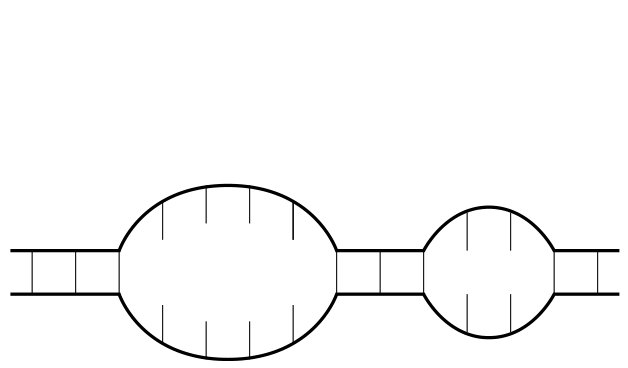
\includegraphics[width=0.9\textwidth]{../assets/2598/PS.png}
\caption{\footnotesize Standard PS model.}\label{fig:PS}
\end{subfigure}
\qquad \qquad
\begin{subfigure}[t]{0.4\textwidth}
\centering
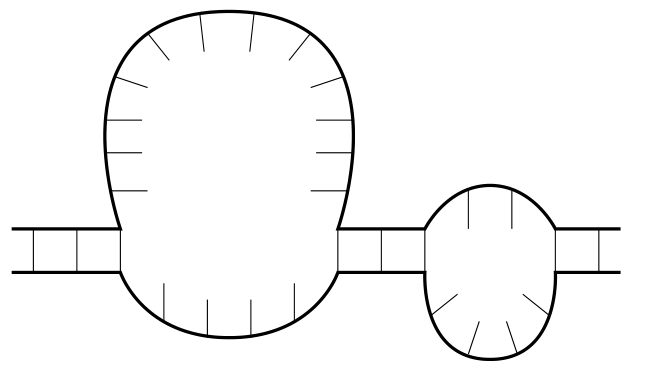
\includegraphics[width=0.9\textwidth]{../assets/2598/gPS.png}
\caption{\footnotesize Generalized PS model.}\label{fig:gPS}
\end{subfigure}
\caption{Standard v. Generalized Poland--Scheraga models. The figure on the left represents the standard PS model: the two strands of DNA have the same length (there are $14$ base pairs in Figure~\ref{fig:1}\eqsubref{fig:PS}), loops are symmetric (there are $5$~loops of lengths $1$, $1$ loop of length $3$ and $1$ loop of length $5$). The figure on the right represents the generalized PS model: the two strands may have a different number of bases ($22$ for the ``top'' one, and $16$ for the ``bottom'' one), and loops are allowed to be asymmetric and can be encoded by two numbers $(n,m)$ %\linebreak
where $n$ is the length the ``top'' strand and $m$ of the ``bottom'' strand (the loops in Figure~\ref{fig:1}\eqsubref{fig:gPS} are from left to right $(1,1),(1,1),(13,5),(1,1),(1,1),(3,5),$ $ (1,1)$).\label{fig:1}}
\end{figure}



A remarkable feature of the non disordered PS model (this corresponds to the case in which all the bases are the same: for example a strand AAA\dots and a second strand TTT\dots) is its solvable character. Notably, one can show that the model has a \emph{denaturation} transition in the limit of infinite strand length, and one can identify the critical point (the critical temperature) and the critical behavior, i.e. the nature of the singularity of the free energy at the critical value. Somewhat surprisingly, also the gPS model is exactly solvable, in spite of the fact that it is considerably more complex than the PS model. This has been pointed out first in~\cite{cf:GOO,cf:GO04,cf:NG06} and a mathematical treatment can be found in~\cite{cf:GK}. Let us stress that the higher complexity level of the gPS model is however reflected in a richer behavior. Notably, in the gPS model, other phase transitions exist, beyond the denaturation transition. Another relevant remark is that PS and gPS models contain a parameter (the \emph{loop exponent}) that, in a mathematical or theoretical physics perspective, can be chosen arbitrarily and on which depends the critical behavior. In fact in this class of models the critical exponent depends on this parameter, and arbitrary critical exponents can be observed by tuning the loop exponent.


Stepping to the disordered model is not (at all) straightforward. One way to attack the problem is by looking at it as a stability issue: is the transition (and we will focus on the denaturation one) still present in the model if we introduce some disorder, for example a small amount? And, if it does, what is the new critical value and is the critical behavior the same as without disorder? We refer to~\cite[Chapter~5]{cf:GB} for an outline on this general very important issue in statistical mechanics and on the renormalization group ideas that lead to the so called \emph{Harris criterion} of disorder irrelevance. We speak of disorder relevance when the disorder, irrespective of its strength, makes the critical behavior of the model different from the one of the non disordered model. Disorder is instead irrelevant if the two critical behaviors coincide for a small disorder strength. In the relevant (resp. irrelevant) case one can argue that applying a coarse graining procedure makes the disorder stronger (resp. weaker). Harris' idea is that disorder (ir)relevance, can be read out of the critical exponent in the non disordered model.

More precisely, Harris criterion says that, if $\nu$ denotes the correlation length exponent of the non-disordered system and $d $ the dimension, $\nu >2/d$ implies disorder irrelevance, at least if the disorder is not too strong. One also expects disorder relevance if $\nu< 2/d$. The case $\nu= 2/d$ is dubbed marginal and deciding whether disorder is relevant or not is usually a delicate issue, even leaving aside mathematical rigor. The PS and gPS models, with their wide spectra of critical behaviors, therefore become an ideal framework for testing the validity of the physical predictions. In fact, the mathematical activity on the PS model (which is one-dimensional) has been very successful. Results include:
\begin{itemize}
\item Very complete understanding of the PS model when disorder is irrelevant\linebreak\cite{cf:A08,cf:G,cf:Lac,cf:Ton08};
\item Precise estimates on the disorder induced shift of the critical point (with respect to the annealed model) in the relevant disorder case~\cite{cf:AZ09,cf:DGLT09}, and a proof of the fact that disorder does change the critical exponent~\cite{cf:CH13,cf:GT06} (without determining the new one: this is an open problem also in the physical literature, even if consensus is starting to emerge about the fact that pinning model in the relevant disorder regime should display a very smooth localization transition, see~\cite{cf:BGL,cf:DR} and references therein);
\item Determination of whether or not there is a disordered induced critical point shift in the marginal case, and precise estimates of this shift: this issue was controversial in the physical literature~\cite{cf:BL16,cf:1GLT10}. In absence of critical point shift, the critical exponent has also been shown to be unchanged by the noise. Showing that disorder does change the critical behavior when there is a critical point shift at marginality is an open issue, and determining the critical behavior in presence of disorder does not appear to be easier than attacking the same issue in the relevant case~\cite{cf:DR}.
\end{itemize}

Our aim is to analyze the disordered gPS model and to understand the effect of disorder on the denaturation transition for this generalized, 2--dimensional, model.

\subsection{The generalized Poland--Scheraga model}\label{sec:model}

Let $\tau = {\lbrace \tau_n \rbrace}_{n\geq 0}= {\lbrace (\tau_n^{(1)}, \tau_n^{(2)}) \rbrace}_{n\geq 0}$ to be a bivariate renewal process, i.e. $\tau_0 = (0,0)$ and $\{ \tau_{n} - \tau_{n-1}\}_{n \geq 1}$ are identically distributed $\mathbb{N}^2$--valued random vectors. We denote by $\bP$ the law of $\tau$, and we assume that it has inter-arrival distribution\linebreak $\bP(\tau_1= (n,m))= K(n+m)$, where
%~ pas de césure avant les opérateurs en mode texte
\begin{equation}\label{def:Kn}
K(n) := \frac{L(n)}{n^{2+\ga}}\,,
\end{equation}
for some $\ga \ge 0$ and some slowly varying function $L({\,\cdot\,})$. Let $\mu := \bE [\tau_1^{(1)}]= \bE [\tau_1^{(2)}]\in (1, \infty]$. Without loss of generality, we assume that $\tau$ is persistent, i.e. $\sum_{n,m} K(n+m) =1$. A set $\tau={\lbrace \tau_n \rbrace}_{n\geq 0}$ is then interpreted as a two-strand DNA configuration: the $\tau_n^{(1)}$'s monomer of the first strand is attached to the $\tau_n^{(2)}$'s monomer of the second strand. Put differently, the $n^{\tHt}$ loop in the double strand is encoded by $(\tau_n^{(1)}-\tau_{n-1}^{(1)},\tau_n^{(2)}-\tau_{n-1}^{(2)})$, see Figure~\ref{fig:PS} and its caption. We refer to~\cite{cf:GK} for further details.

Let $ \omega := { \lbrace \omega_{n,m} \rbrace }_{n,m \in \bbN}$ be a sequence of IID centered random variables (the disorder), taking values in $\bbR$, with law denoted $\bbP$. We assume that the variables $\omega_{n,m}$ are centered, have unit variance and exponential moments of all order, and we set\linebreak for $\beta \in \bbR$
\begin{equation}\label{eq:defQ}
Q(\beta) := \bbE [\exp(\beta \omega)] < \infty\,.
\end{equation}
This choice of disorder is discussed in detail in Section~\ref{sec:misc}.

Given $\beta >0$, $h \in \bbR$ (the pinning parameter) and $N,M \in \bbN$, we define $\bP_{N,M}^{\beta,h,\omega}$ a measure whose Radon--Nikodym derivative w.r.t. $\bP$ is given by
\begin{equation}
\frac{\dd \bP_{N,M,\omega}^{\beta,h}}{\dd \bP} (\tau) := \frac{1}{Z_{N,M, \omega}^{\beta,h}} \exp \!\left(\sum_{n=1}^N \sum_{m=1}^M (\beta \omega_{n,m}+h) \unbf_{(n,m) \in \tau} \right)\! \unbf_{(N,M)\in \tau}\,,
\end{equation}
where $Z_{N,M,\omega}^{\beta,h}$ is the constrained partition function (the normalization constant)
\begin{equation}\label{eq:pf}
Z_{N,M,\omega}^{\beta,h} := \bE \left[\exp\! \left(\sum_{n=1}^N \sum_{m=1}^M (\beta \omega_{n,m} +h) \unbf_{(n,m) \in \tau} \right)\! \unbf_{(N,M)\in \tau} \right].
\end{equation}
This corresponds to giving a reward $\gb \go_{n,m}+h$ (or a penalty if it is negative) if the $n^{\tHt}$ monomer of the first strand and the $m^{\tHt}$ monomer of the second strand meet. Note that the presence of $\unbf_{(N,M)\in \tau}$ in the right-hand side means that we are considering trajectories that are pinned at the endpoint of the system (at a technical level it is more practical to work with the system pinned at the endpoint, see the proof of Theorem~\ref{th:fq}). Note that, by definition, there are at most $\min (N,M)$ renewals in the region $\{1,\ldots, N\}\times \{1,\ldots, M\}$.

We also define the \emph{free} partition function, where the endpoints are free
\begin{equation}\label{eq:free}
Z^{f,\beta,h}_{N,M,\omega}= \bE \left[\exp \!\left(\sum_{n=1}^N \sum_{m=1}^M (\beta \omega_{n,m} +h) \unbf_{(n,m) \in \tau} \right) \right],
\end{equation}
that can be compared to the \emph{constrained} partition function~\eqref{eq:pf}, see Lemma~\ref{th:zfc}. For notational convenience, we will sometimes suppress the $\beta,h$ from the partition function.

%%\smallskip

One then defines the \emph{quenched} free energy of the system. We prove the following theorem in Section~\ref{sec:existence}.

\begin{theo}\label{th:fq}
For all $\gamma>0$, $h \in \bbR$, $\beta \ge 0$ and every choice of $\{M(N)\}_{N=1,2, \ldots}$ such that $\lim_{N\to\infty} M(N)/N=\gamma$ we have
\begin{equation}\label{eq:saf}
\lim_{N\to\infty} \frac{1}{N} \log Z^{\gb,h}_{N,M(N),\omega} = \lim_{N\to\infty} \frac{1}{N} \bbE \log Z^{\gb,h}_{N,M(N),\omega} =: \tf_{\gamma}(\beta,h)\,,
\end{equation}
where the first limit exists $\bbP(\dd \go)$-almost surely and in $L^1(\bbP)$. The same result holds for the free model, that is $\tf_{\gamma}(\beta,h) = \lim_{N\to\infty} \frac{1}{N} \log Z^{f,\gb,h}_{N,M(N),\omega}$ $\bbP(\dd \go)$-a.s. and in~$L^1(\bbP)$.

The function $(\gb,h) \mapsto \tf_{\gamma}(\gb,h)$ is convex, $h\mapsto \tf_{\gamma}(\gb,h)$ and $\gb\mapsto \tf_{\gamma}(\gb,h)$ are nondecreasing, and $\gamma \mapsto \tf_{\gamma}(\gb,h)$ is nondecreasing and continuous.
\end{theo}

The homogeneous model corresponds to the case $\beta = 0$: let us drop the $\gb$ and $\go$ dependence in the partition function that will be simply denoted $Z_{N, M}^h$.\linebreak The homogeneous model is \emph{exactly solvable} and sharp estimates of $\tf_\gamma (0,h)$ near criticality are given in~\cite{cf:GK}.

\begin{theo}[\cite{cf:GK}]\label{th:beta0}
For every $\gamma \ge 1$, when $\beta=0$ we have $h_c(0) := \sup\{ h\,:\,\tf_{\gamma}(0,h)=0\}= 0$. Moreover there is a slowly varying function $L_{\ga, \gamma}({\,\cdot\,})$ such that as $h \searrow 0$ one has
\begin{equation}
\tf_\gamma (0,h) \sim L_{\ga,\gamma} (h)\,h^{1/ \min (1, \ga)}\,.
\end{equation}
Moreover, if $\sum_n n^2 K(n) \!<\! \infty$ (i.e. $\mu\!<\!\infty$), then ${L_{\ga,\gamma}(h)}^{-1} \Mk\!=\! c^{-1} \!\Mk:=\! \frac{1}{2} \sum_{n } n(n\!-\!1) K(n)$.
\end{theo}

%%\noindent
In fact, the disordered system also presents this transition: we define the critical point
\begin{equation}
h_c(\beta) := \sup \lbrace h\,:\,\tf_\gamma (\beta,h) = 0 \rbrace = \min \lbrace h\,:\,\tf_\gamma (\beta,h) >0 \rbrace\,.
\end{equation}
Let us note that $h_c(\gb)$ does not depend on $\gamma >0$, thanks to~\eqref{eq:existence+.3} below.

On the other hand, we define the annealed free energy as
\begin{equation}
\tf_\gamma^{a}(\beta,h) := \limtwo{N\to\infty,}{M(N) / N \to \gamma} \frac{1}{N} \log \bbE Z_{N,M(N),\omega}^{\gb,h} = \tf_\gamma (0, h + \log Q(\beta))\,.
\end{equation}
This link with the homogeneous model and the fact that $h_c(0)=0$ allow immediately to identify the annealed critical point:
\begin{equation}\label{eq:hann}
h_c^{a}(\beta) := \min \lbrace h\,:\,\tf^{a}_\gamma (\beta,h) >0 \rbrace = - \log Q(\beta)\,.
\end{equation}
Now observe that by Jensen's inequality, we have that $\bbE \log Z_{N,M,\omega} \le \log \bbE Z_{N,M,\omega}$ and hence $\tf_\gamma^{q}(\beta,h) \le \tf_\gamma^{a}(\beta,h)$. Moreover, since $\beta \mapsto \tf_\gamma (\beta,h)$ is non-decreasing, we have that $\tf_\gamma (0,h) \le \tf^{q}_\gamma (\beta,h) $. Therefore for every $\beta$ we have
\begin{equation}\label{eq:inh}
h_c^{a}(\beta)\le h_c(\beta) \le h_c(0)\,.
\end{equation}
One can show, by adapting the argument of proof of~\cite[Theorem~5.2]{cf:G}, that the second inequality is strict for every $\gb \neq 0$. The first inequality may or may not be strict and this is an important issue which is directly linked to disorder relevance and irrelevance.


%%\smallskip
Harris' criterion predicts that disorder is irrelevant if $\nu>2/d$. Here, Theorem~\ref{th:beta0} suggests that $\nu=1/\min(1,\alpha)$, if we admit that the correlation length of the non-disordered system can be given by the reciprocal of the free energy, as it is the case for the PS model, see~\cite{cf:G08}. Since the model is $2$-dimensional (contrary to the PS model which is $1$-dimensional), it would mean that disorder is irrelevant when $\nu>1$, that is when $\ga<1$.



And in fact our first result states that the first inequality in~\eqref{eq:inh} is an equality if $\ga<1$ and $\gb$ is not too large. For the same values of $\gb$ we can also show that the critical behavior is the same as for the $\gb=0$ case (disorder irrelevance). Our second result asserts that the inequality is strict for $\ga>1$. We interpret this critical point shift, with a certain abuse, as disorder relevance. We however refer to the discussion in Section~\ref{sec:misc} (in particular Conjecture~\ref{conj:smoothing}) regarding the change in the critical behavior. We therefore prove that disorder is irrelevant if $\ga<1$, and relevant\linebreak(in terms of critical points) if $\ga>1$, confirming Harris' prediction.



\subsection{Relevance and irrelevance of disorder}

Let us define $\sigma :=\tau \cap \tau'$, where~$\tau$ and~$\tau'$ are two independent copies of~$\tau$: $\sigma$ is another bivariate renewal process, and Proposition~\ref{prop:transience} tells that $\sigma$ is terminating if $\ga\in(0,1)$ and persistent if $\ga>1$ (the case $\ga=1$ is discussed in Remark~\ref{rem:alpha=1}).


\begin{theo}\label{thm:irrel}
Assume that $\sigma$ is terminating (this includes $\ga<1$ and excludes $\ga >1$). Then there exists $\beta_1>0$ (see~\eqref{eq:beta1}), such that for every $\beta \in (0,\beta_1)$ we have $h_c(\beta) = h_c^a(\beta)$, and moreover
\begin{equation}\label{eq:s2}
\lim_{h \searrow h_c(\beta)} \frac{\log \tf_{\gamma}(\beta,h)}{\log (h-h_c(\beta))} = \frac{1}{\ga}\,.
\end{equation}
\end{theo}

Hence, the order of the phase transition is unchanged when $\sigma$ is terminating (which is the case if $\ga<1$), at least when $\gb$ is small enough. We prove Theorem~\ref{thm:irrel} in Section~\ref{sec:irrel}. We mention that when the disorder distribution is infinitely divisible (for instance Gaussian), one can get sharper bounds regarding the critical behavior of $\tf_{\gamma}(\beta,h)$, via a replica-coupling method, as done in~\cite{cf:Ton08} or~\cite{cf:Wa12}. For a statement and a detailed proof, we refer to~\cite{cf:Khatib}.

On the other hand, when $\ga>1$, we show that the quenched and annealed critical points differ, and we give a lower bound on the critical point shift.

%%\medskip
\begin{theo}\label{thm:rel}
For $\ga>1$ we have $h_c(\gb) > h_c^{a}(\gb)$ for every $\beta>0$. Moreover, for every $\gep>0$, there exists $\gb_{\gep}>0$ such that for any $\gb\leq \gb_\gep$ we have
\begin{equation}\label{eq:rel}
h_c(\beta) - h_c^{a}(\beta)\ge \gD_{\gb}^{\gep}:=
\begin{cases}
\gb^{\frac{2\ga}{\ga-1} +\gep} & \text{if } \ga\in(1,2]\,, \\
\gb^4 \mathopen|\log \gb |^{-6} & \text{if } \ga >2\,.
\end{cases}
\end{equation}
Moreover, there is a slowly varying function $\tilde{L}({\,\cdot\,})$ such that
\begin{equation}\label{eq:upb}
h_c(\beta) - h_c^a (\beta) \le
\tilde{L}(1/\gb) \gb^{\frac{2\ga}{\ga-1} \vee 4}\,.
\end{equation}
\end{theo}

%%\medskip
We add that $\gb\mapsto h_c(\gb)-h_c^{a}(\gb)$ is a non decreasing function of $\beta$: this result can be proven by the exact same procedure as the one used to prove in~\cite[Proposition~6.1]{cf:GLT11}. It is to be interpreted that disorder relevance is \emph{non-decreasing} in~$\beta$.

\subsection{On the results, perspectives and related work}\label{sec:misc}

\subsubsection{On the main theorems}

A two replica computation plays a central role in the proof of Theorem~\ref{thm:irrel} and in the proof of~\eqref{eq:upb} of Theorem~\ref{thm:rel}: the intersection renewal $\sigma$ therefore emerges naturally, like in the PS model. In the PS context, we now know that disorder is irrelevant (for small values of $\gb$) if and only if the intersection renewal is terminating~\cite{cf:BL16}. For the gPS model our results go in the same direction, but it is not sharp in the marginal case $\ga=1$: we only show disorder irrelevance when the intersection renewal $\sigma$ is terminating. We refer to Remark~\ref{rem:alpha=1} for further discussion on the case $\ga=1$, where more technicalities arise.

The proof of~\eqref{eq:rel} is based on coarse graining techniques and fractional moment method: we have chosen to adapt the method proposed in~\cite{cf:DGLT09} and the difficulties in its generalization come from dealing with the richness of a multidimensional path with respect to the one dimensional structure of the PS models. A keyword for these difficulties is \emph{off-diagonal estimates}. It can certainly be improved in the direction of getting rid of the~$\gep$ in the exponent for $\ga \in (1, 2]$ and of the logarithmic term in the case $\ga >1$ by using more sophisticated coarse graining techniques (see~\cite[Chapter~6]{cf:G} and references therein). One could probably aim also for sharp estimates, like in~\cite{cf:BL16}, but the estimates are technically rather demanding already to obtain~\eqref{eq:rel}. We have chosen to stick to these simplified non-optimal (but almost optimal) bounds because sharper results would have required a substantially heavier argument of proof. The techniques developed in~\cite{cf:BL16bis,cf:BL16} should transfer to this model: at the expense of a high level of technicality, we expect that, in analogy with the PS model, the necessary and sufficient condition for a critical point shift is the persistence of the intersection renewal $\sigma=\tau\cap\tau'$.

\subsubsection{Discussion on the presence of a \emph{smoothing} phenomenon}

Of course, a fully satisfactory result on disorder relevance would include showing that the critical exponent is modified by the disorder. We do not have such a result, but let us make one observation and formulate a conjecture.

The observation is that Theorem~\ref{thm:irrel} may appear at first surprising in view of the smoothing Inequality~\cite{cf:CH13,cf:GT06} for PS models that ensures that the free energy exponent cannot be smaller than $2$ in presence of disorder: for the gPS model the free energy exponent can go down to $1$, since in~\eqref{eq:s2} we can choose $\ga$ arbitrarily close to $1$. The reason of the difference is that the PS model is\linebreak$1$--dimensional whereas the gPS model is $2$--dimensional: Harris criterion tells that disorder should be irrelevant if $\nu>2$ for the PS model, and $\nu>1$ for the gPS model. In the gPS model, the irrelevant disorder regime therefore holds even if $\nu $ ($=\min(1,\ga)^{-1}$) is arbitrarily close to $1$: hence one should not hope for a general smoothing inequality valid whatever $\alpha$ is.

It is however worthwhile attempting to sketch the argument in~\cite{cf:GT06}, in the simplified set-up of Gaussian charges~\cite[Chapter~5, Section~4]{cf:GB}. This is useful both to understand were the argument fails and because we can realize that a suitable generalization of the argument naturally leads to a conjecture that we state just below.

%~ SCfigure n'est pas dans la maquette
%~ Il ya avait aussi un problème de style avec la légende (pas identique à celle des figures ordinaires)
\begin{figure}[htbp]
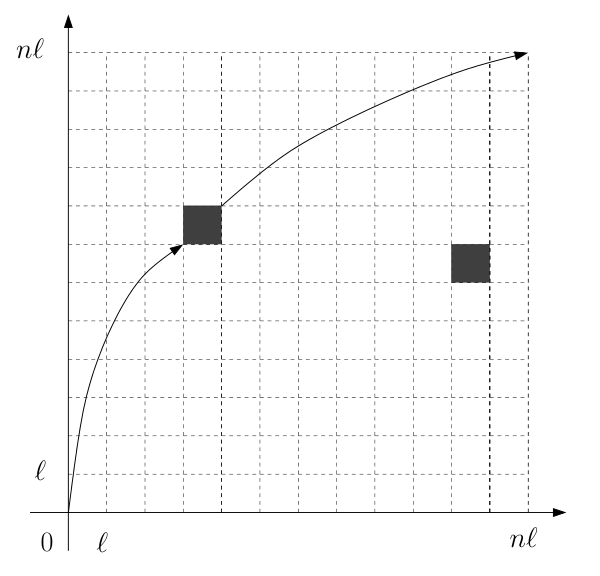
\includegraphics[scale=0.34]{../assets/2598/forSmoothing.png}
\centering
\caption{\label{fig:smoothing}
Schematic view of the coarse graining procedure proposed for a smoothing inequality. The environment is divided in blocks of size $\ell$, called %\linebreak
$\ell$--boxes. A $\ell$--box is good (shadowed in the figure) if the partition function in this block grows at an exponential rate that is larger than the free energy of the system. The good $\ell$--boxes will be rare, but we can choose $n$ such that in a system of linear size $n\ell$, with positive probability, there will be at least one good $\ell$--box. A lower bound on the partition function follows by the limitation to trajectories that visit only a given good $\ell$--box (say, the closest).}
\end{figure}

%\pagebreak
The argument~\cite{cf:GT06} is based on introducing a coarse graining scale $\ell \in \bbN$ and considering the environment in terms of $\ell$-boxes, see Figure~\ref{fig:smoothing}. We argue for the case $\gamma=1$ ($M=N$) and we consider the system at criticality, that is $h=h_c(\gb)$:
\begin{enumerate}
\item A good $\ell$--box is a box for which the pinned partition function (i.e. the renewal is pinned at the south-west and north-east corners of the $\ell$--box) is larger than $\exp(\tfrac12\,\ell\,\tf_1(\gb, h+ \gd))$, with $\gd>0$. For $\ell\to \infty$ this is a rare event. The probability of such an event can be estimated from below by shifting the environment of $\gd/\gb$, that is $\go_{i,j}$ is replaced with $\go_{i,j}+ \gd/\gb$, and by performing a relative entropy estimate~\cite[Chapter~5]{cf:G}. This shows that the probability of such a rare event is at least $\exp(-\gd^2 \ell^2 /(2 \gb^2))$: note the $\ell^2$ term, with respect to $\ell$ in the PS case~\cite{cf:GT06}.
\item We then make a lower bound on the partition function of the system by discarding renewal trajectories that visit $\ell$--boxes that are not good, and keeping only trajectories that enter good $\ell$--boxes through the south-west corner and exit through the north-east corner.
\end{enumerate}


The trajectories are therefore alternated jumps to a good box, \emph{visit} of the box, and then a new jump to another good box. Jumps are long because good boxes are rare. The analysis in~\cite{cf:GT06} is ultimately reduced to see what happens in one \emph{jump and visit}: by exploiting super-additivity one can even just choose $N=n\ell$ such that there is (say, with probability at least $1/2$), at least one good box in the system (like it is done in~\cite{cf:BL11}). We therefore see that we need $n^2 \exp(-\gd^2 \ell^2 /(2 \gb^2))\approx 1$, so that $n \approx \exp(-\gd^2 \ell^2 / \gb^2)$: with this level of precision, jumping to enter such a box costs $K(n\ell) = (n\ell)^{-(2+\ga)}$ (let us consider the case in which $L({\,\cdot\,})$ is a constant, but the computation goes through in the same way also in the general case). In the box there will be a contribution $\exp\big(\tfrac12\,\ell\,\tf_1(\gb, h+ \gd) \big)$. The net contribution to the logarithm of the partition function, divided by the size $n\ell$ of the system, is then
\begin{equation}
\!\frac{1}{n \ell} \!\left(\log K\!\left(\exp(-\gd^2 \ell^2 / \gb^2) \ell \right)\!+\! \frac{\ell}{2} (\tf_1(\gb, h\!+\! \gd))\! \right) \Mk\ge\Mk \frac {1}{n} \!\left(-\frac{c}{\gb^2}\gd^2 \ell\!+\! \frac{1}{2} \tf_1(\gb, h\!+\! \gd)\! \right),\!
\end{equation}
%~condensé pour que ça rentre page 9
with $c$ a positive constant that we have left implicit (it depends on more accurate computations, and can be in principle just reduced to $2+ \ga$).

%\goodbreak
Now let us choose $h=h_c(\gb)$. So the argument we just outlined goes in the direction of saying that
\begin{equation}
0 = \tf_1(\gb, h_c(\gb)) \ge \frac{1}{n} \left(-\frac{c}{\gb^2} \gd ^2 \ell+ \frac{1}{2} \tf_1(\gb, h_c(\gb)+ \gd) \right),
\end{equation}
so that
\begin{equation}
\tf_1(\gb, h_c(\gb)+ \gd)\le \frac{2c}{\gb^2} \gd ^2 \ell\,.\label{eq:tf1sm}
\end{equation}
At this stage choosing $\ell$ arbitrarily large is of no help. The steps we have performed up to now require that $ \ell \gd$ is large (so that the good boxes we have chosen are really sparse). On the other hand we need to have chosen the size of the boxes so that $Z_{\ell, \ell, \go}^{\gb, h} \ge \exp(\ell (\tf_1(\gb, h_c(\gb)+ \gd))/2)$. This is a delicate issue, but it definitely appears that for this to hold, $\ell \tf_1(\gb, h_c(\gb)+ \gd)$ needs to be sufficiently large (say, larger than a suitable constant): see for example the discussion on the notion of correlation length given in~\cite[Chapter~2]{cf:G} and references therein, notably~\cite{cf:GTalea}, where the correlation length is identified by the reciprocal of the free energy. But if $\ell$ is\linebreak(a constant times) $1/\tf_1(\gb, h_c(\gb)+ \gd)$ then from~\eqref{eq:tf1sm} we obtain
\begin{equation}\label{eq:trivb}
\tf_1(\gb, h_c(\gb)+ \gd)\le C \gd\,,
\end{equation}
for some $C>0$. But such a bound is trivial: it holds with $C=1$ just because the contact density cannot exceed one! On the other hand, as we have already pointed out, we could not have hoped for a better bound valid for any $\alpha>0$.

%%\smallskip
In spite of the fact that it leads to a trivial result, we insist that the argument we have just outlined can be made rigorous: the delicate step is the last one, where one has to use arguments developed in~\cite{cf:GTalea}. It can therefore be taken as a starting point to push things further. Indeed, it appears useless to modify the environment in the whole $\ell$--box, at least if $\ga>1$. In fact if $\ga>1$ one can show that for $q>1/ \max(\ga,2)$
\begin{equation}\label{eq:evin}
\lim_{N \to \infty}\bP \left(\tau \cap [0, N]^2 \subset \{(i,j) \in \bbZ^2:\,\vert i-j \vert \le N^q \}\right)= 1\,.
\end{equation}
We can then consider modifying only the environment that is close to the diagonal, that is in a subset of the $\ell$-box with $|i-j|\leq \ell^q$. This would improve the lower bound on the probability of a good $\ell$-box to $\exp(- c'\,\gd^2 \ell^{q+1})$, and~\eqref{eq:tf1sm} would become
\[
\tf_1(\gb,h_c(\gb)+\gd) \leq \frac{c''}{\gb^2} \gd^2 \ell^{q}.
\]
Taking $\ell$ a constant times $1/\tf_1(\gb,h_c(\gb)+\gd)$ as in the argument leading to~\eqref{eq:trivb}, and then taking $q$ arbitrarily close to $1/\min(\alpha,2)$ supports the following:
\begin{conj}
For every $\ga>0$ and every $\gb >0$\label{conj:smoothing}
\begin{equation}
\limsup_{\gd \searrow 0} \
\frac{\log \tf_1 (\gb, h_c(\gb)+\gd) }{\log \gd}\ge
\begin{cases}
\frac{2\ga}{\ga+1} & \text{ for } \ga \in (1,2)\,,
\\
\;\:\frac{4}{3} & \text{ for } \ga \ge 2\,.
\end{cases}
\end{equation}
\end{conj}

We stress that a natural concern arises from performing the change of measure only in a subset of the environment, close to the diagonal. One indeed needs to be sure that the trajectories contributing to (a fraction of) $ \frac{1}{\ell} \log Z_{\ell,\ell,\go} \approx \tf_1(\gb,h_c(\gb)+\gd)$ can be constrained to stay in the region $\{(i,j) \in \bbZ^2:\,\vert i-j \vert \le \ell^q \}$: if it is the case, one can ``force'' trajectories to visit sites where the environment has indeed been shifted.

\subsubsection{An important modeling issue: the choice of the disorder}

There is no doubt that the first disorder that comes to mind when thinking of DNA modeling is not the one we have used. One would rather choose $\go_{i,j}=f(\go_i, \go_j)$ for a suitable choice of a function $f$ and a sequence $\{\go_j\}_{j=1,2, \ldots}$ of random variables (let us say IID for simplicity, but if we want to stick to DNA problems very closely it appears that some sort of strongly correlated sequence may be more appropriate~\cite{cf:Peng}). For example, we could choose $\go_j$ taking only two values $e_{AT}$ and $e_{GC}$ and then make a choice for $f$ that reflects the fact that AT bounds are weaker than GC bounds, and that all other possible bounds are even weaker. Even restricting to $\{\go_j\}_{j=1,2, \ldots}$ that is IID, this model is highly non trivial (gPS model with this type of disorder has been considered at a numerical level in~\cite{cf:GOO,cf:GO04}, see also~\cite{cf:EON11,cf:TN08} for related work). But one could also choose to consider the binding of two sequences that are not complementary (the case considered in~\cite{cf:NG06} goes in this direction, even if only heuristics and numerics are presented): choose for example two independent sequences $\{\go^{(1)}_j\}_{j=1,2, \ldots}$ and $\{\go^{(2)}_j\}_{j=1,2, \ldots}$ and use $\go_{i,j}=f(\go^{(1)}_i, \go^{(2)}_j)$. This is somewhat closer to what we are using (though it can be considered as a one-dimensional disorder), but it is still very difficult to deal with. The problem is in any case due to correlations in the disorder field $\go_{i,j}$, which can be dealt with in some cases, see e.g.~\cite{cf:BL12,cf:BP15} or~\cite{cf:AB18, cf:CCP17}. Our choice is in a sense a toy choice, but we stress that it is conceptually similar to the simplification made for example in~\cite{cf:BundHwa} in the RNA context. Moreover it recovers importance once we leave somewhat the DNA context and focus rather on moving toward understanding mathematically Harris' theory of disorder (ir)relevance--in particular for 2--dimensional systems, compared to the PS model, which is 1-dimensional.

We also point out that this disordered version of the gPS model gives a bridge between pinning model and directed polymers in random environment~\cite{cf:Co07,cf:La10}, in particular, to the long range directed polymer~\cite{cf:Co07,cf:We15}. Moreover a different class of two-strand polymer problems (the random walk pinning model) is treated in~\cite{cf:BS1,cf:BS2,cf:BT10}.

\subsubsection{Open questions and perspectives}

Several natural issues remain open: let us list some of them.
\begin{enumerate}
\item Prove a smoothing inequality, thus showing disorder relevance in the original sense of Harris, for $\ga>1$ (see Conjecture~\ref{conj:smoothing}).
\item What is the effect of disorder on the other phase transitions? Here we have addressed only the denaturation transition, but in~\cite{cf:GK} other transitions are shown to exist. Do they withstand the introduction of disorder? If so, does the corresponding critical behavior differ from the homogeneous case? This is the question (quickly) addressed~\cite{cf:NG06} where a rather bold conjecture is set forth.
\item We have dealt only with free energy estimates, but, like for the standard PS model, obtaining precise estimates on the gPS process (i.e. establish properties of trajectories) is very challenging, see~\cite[Chapter~8]{cf:G} and references therein. The problem comes of course from the inhomogeneous nature of the disorder and the fact that on rare regions atypical disorder behaviors appear (this is ultimately also the problem we face at the free energy level, but it becomes particularly explicit when one analyses the trajectories). A precise analysis of the trajectories of the non disordered gPS model can be found in~\cite{cf:BGK}: this analysis is substantially more demanding than the corresponding one for the PS model.
\item Dealing with the marginal case $\ga=1$ is open, mostly because of the additional technical difficulties (more complicated coarse-graining procedure, more technical estimates for bivariate renewals, etc.). This appears to be a problem at reach, but a very substantial amount of technical work is certainly needed.
\end{enumerate}

\subsubsection{Organization of the rest of the work}

The issues of existence and self-averaging of the free energy, i.e. the proof of Theorem~\ref{th:fq}, are treated in Section~\ref{sec:existence}. In Section~\ref{sec:irrel} we prove Theorem~\ref{thm:irrel}, as well as the upper bound~\eqref{eq:upb} of Theorem~\ref{thm:rel}. The rest of the Theorem~\ref{thm:rel} is proven in Section~4. We collect in Appendix~\ref{app:bivrenewal} a number of statements and proofs about bivariate renewals.

\subsection{Some further notations}\label{sec:defan}

We stress that $\tau$ is symmetric and in the domain of attraction of a $\min(\ga,2)$-stable distribution: we denote $(b_n)_{n\geq 1}$ be the recentering sequence and ${(a_n)}_{n \ge 0}$ the renormalizing sequence for $\tau_n$, that is such that $\tfrac{1}{a_n} (\tau_n - (b_n,b_n))$ converges to a $\min(\ga,2)$ stable distribution, whose density is denoted $g_\ga({\,\cdot\,,\cdot\,})$. For $b_n$, we have $b_n=\mu n$ if $\ga>1$, $b_n= n\bE[\min(X_1, n)]$ if $\ga=1$, and $b_n=0$ if $\ga \in(0,1)$. The asymptotic behavior of $a_n$ is characterized by
\begin{equation}\label{def:an}
\begin{cases}
L(a_n) (a_n)^{-\ga} \sim 1/n &\text{if } \ga<2,\\
\,\sigma(a_n) (a_n)^{-2} \sim 1/n &\text{if } \ga\geq 2,
\end{cases}
\end{equation}
where $\sigma(n):=\bE[\min(X_1, n)^2]$. If $\ga = 2$ and $\bE[X^2]=+\infty$, then $\sigma(n)$ grows to infinity as a slowly varying function (and verifies $\sigma(n)/L(n) \to +\infty$), whereas if $\bE[X^2]<+\infty$ (in particular when $\ga>2$) $a_n$ is proportional to $\sqrt{n}$.

In any case, there exists some slowly varying function $\psi({\,\cdot\,})$ such that
\begin{equation}
a_n = \psi(n) n^{1/\min(\ga, 2)}\,.\label{an}
\end{equation}
We provide some useful results on bivariate renewals in Appendix~\ref{app:bivrenewal}, in particular on the renewal mass function $\bP((n,m)\in\tau)$.


\section{Free Energy: existence and properties}\label{sec:existence}

In this section we often assume $\gamma\in \bbQ$: in this case we write it as $\gamma=p/q$ with $p$ and $q$ relatively prime positive integer numbers.


\begin{prop}\label{th:existence+}
For every $\gamma>0$ and every $\{M(N)\}_{N=1,2, \ldots}$ such that $\lim_{N \to \infty} M(N)/N=\gamma$ we have that
\begin{equation}\label{eq:existence+.1}
\lim_{N \to \infty} \frac{1}{N} \log Z_{N,M(N), \go}^{\gb,h}= \lim_{N \to \infty}
\frac{1}{N} \bbE \log Z_{N,M(N), \go}^{\gb,h} =: \tf_\gamma(\gb, h)\,,
\end{equation}
where the first limit is meant $\bbP(\dd \go)$-a.s. and in $L^1 (\bbP)$. $\tf_\gamma ({\,\cdot\,,\cdot\,})$ is convex and $\tf_\gamma ({\gb,\cdot\,})$ is non-decreasing, and also $\tf_\gamma ({\,\cdot\,,h})$ is non-decreasing on the positive semi-axis, non-increasing in the negative one. Moreover if $\gamma=\frac{p}{q}\in \bbQ$
\begin{equation}\label{eq:existence+.2}
\tf_\gamma (\gb, h) = \sup_{N:\,\frac{N}{q}\in \bbN} \frac{1}{N} \bbE \log Z_{N, \gamma N, \go}^{\gb,h}\,.
\end{equation}
Finally we have the bound: for every $\gamma_2\ge \gamma_1 >0$
\begin{equation}\label{eq:existence+.3}
\tf_{\gamma_1}(\gb, h) \le \tf_{\gamma_2}(\gb, h)\le \frac{\gamma_2}{\gamma_1} \tf_{\gamma_1}(\gb, h)\,,
\end{equation}
which implies that $\gamma \mapsto \tf_{\gamma}(\gb, h)$ is locally Lipschitz (hence continuous).
\end{prop}

%%\noindent
\begin{proof}
The proof is divided into several steps:
\begin{enumerate}
\item\label{pr-list-step1} We first show that for $\gamma \in \bbQ$, along a subsequence with $ N/q\in \bbN$, $\log Z_{N, \gamma N, \go}$ is super-additive in an ergodic sense, which implies the existence of the free energy limit~\eqref{eq:existence+.1} along this subsequence.
\item \label{pr-list-step2} The restriction $\gamma N\in \bbN$ is then removed by a direct estimate, for what concerns the existence of the free energy limit, still with $\gamma \in \bbQ$.
\item \label{pr-list-step3}We then prove a comparison estimate between $Z_{N, \gamma_1 N, \go}$ and $Z_{N, \gamma_2 N, \go}$ and use it to establish the existence of the free energy limit for $Z_{N, \gamma N, \go} $, every $\gamma>0$.
\item \label{pr-list-step4}The same comparison estimate yields also~\eqref{eq:existence+.3}, and the fact that one can take the limit along an arbitrary sequence satisfying $M (N) \sim \gamma N$, for $N \to \infty$.
\item \label{pr-list-step5}Finally, we prove the convexity and monotonicity statements.
\end{enumerate}
\goodbreak

%%\noindent
\begin{step}{Step~(\ref{pr-list-step1})}
With $\gamma=p/q$ set $
\cZ_{j}(\go) := Z_{jq, jp, \go}$. Then one directly sees that
\begin{equation}\label{eq:super-add-erg}
\cZ_{j_1+j_2}(\go)\ge \cZ_{j_1}(\go) \cZ_{j_2}\left(\Theta_{j_1 q,j_1 p} \go\right),
\end{equation}
where $(\Theta_{q,p} \go)_{n,m}= \go_{q+n,p+m}$. Since $\go$ is an IID sequence of $L^1$ random variables, it is straightforward to see that $\log \cZ_{j} \in L^1(\bbP)$. Also,
\[
\lvert \log \cZ_{j} \vert \leq h n+ \gb \sup_{\gamma \in \Gamma } \sum_{(n,m)\in\gamma} |\go_{n,m}|,
\]
where $\Gamma$ is the set of nearest-neighbors up-right paths: a Last Passage Percolation observation then tells us that a sufficient condition for having $\sup_n \frac{1}{n} \bbE \lvert\log \cZ_{j} \vert <+\infty$ is $\bbE[\go_{1,1}^2]<+\infty$, see~\cite{cf:Martin02}. Hence we see that $\{ -\log \cZ_{j}(\go)\}_{j=1,2, \ldots}$ satisfies the hypotheses of Kingman sub-additive ergodic Theorem (see for example~\cite[Section~A.7]{cf:GB}), and we get that $\{\frac{1}{j}\log \cZ_{j}(\go)\}_{j=1,2,\ldots}$ converges $\bbP(\dd \go)$-a.s. and in $L^1(\bbP)$. Moreover~\eqref{eq:super-add-erg} directly tells us that $\{\bbE \log \cZ_{j}(\go)\}_{j=1,2, \ldots}$ is super-additive, so that $\lim _{j\to \infty} \frac{1}{j} \bbE \log \cZ_{j}(\go)= \sup_{j\in \bbN} \frac{1}{j} \bbE \log \cZ_{j}(\go)$. This establishes~\eqref{eq:existence+.2}, and also~\eqref{eq:existence+.1}, but only for $M(N)= \gamma N$ with $\gamma \in \bbQ$ and along the subsequence satisfying $\gamma N \in \bbN$.
\end{step}
%% Step

%%\smallskip
\begin{step}{Step~(\ref{pr-list-step2})}
Still with $\gamma =p/q$, the restriction to $\gamma N \in \bbN$ can be removed by observing that we can write $N= jq+r$, with $r\in \{0, 1, \ldots, q-1\}$, and for $r\neq 0$
\begin{equation}\label{eq:exist-step2.1}
\begin{split}
Z_{N, \lfloor \gamma N \rfloor, \go} &\ge Z_{jq, jp, \go} \exp(\gb \go_{N, \lfloor \gamma N \rfloor}+h) K \Big(r+ \Big \lfloor jp+ \frac{p}{q} r \Big \rfloor -jp \Big)
\\ & \ge c(p,q) \exp(\gb \go_{N, \lfloor \gamma N \rfloor}+h) Z_{jq, jp, \go}\,,
\end{split}
\end{equation}
where $c(p,q)>0$.

In the same way
\begin{multline}\label{eq:exist-step2.2}
Z_{(j+1)q, (j+1)p, \go}\\
\begin{aligned}
&\ge Z_{N, \lfloor \gamma N \rfloor, \go} \exp(\gb \go_{(j+1)q, (j+1)p}+h)\,K \Big(q-r+ (j+1)p- \Big \lfloor jp+ \frac{p}{q} r \Big \rfloor\!\Big)\\
&\ge c(p,q) \exp(\gb \go_{(j+1)q, (j+1)p}+h) Z_{N, \lfloor \gamma N \rfloor, \go}\,,
\end{aligned}
\end{multline}
possibly redefining $c(p,q)>0$. From~\eqref{eq:exist-step2.1} and~\eqref{eq:exist-step2.2} one easily removes the restriction to $\gamma N \in \bbN$ and establishes~\eqref{eq:existence+.1} for $M(N) = \lfloor \gamma N \rfloor$ with $\gamma\in \bbQ$.
\end{step}
%%\smallskip

\begin{step}{Step~(\ref{pr-list-step3})}
We now establish~\eqref{eq:existence+.1} for $M(N)= \lfloor \gamma N\rfloor$ for an arbitrary $\gamma>0$, by proving the announced comparison bounds, upper and lower.

The upper bound is more general: if $M_2> M_1$ and if there exists $c>0$ such that $M_2 \le c N$ we see that
\begin{equation}\label{eq:comparison-upper}
\begin{split}
Z_{N, M_1, \go} & = \sum_{n=0}^{N-1} \sum_{m=0}^{M_1-1} Z_{n, m, \go} K(N-n+M_1-m) \exp\left(\gb \go_{N, M_1} +h\right)
\\
&\le c_K N^{c_K} \exp\left(\gb (\go_{N, M_1}-\go_{N, M_2}) \right)
\\ & \quad \qquad \times
\sum_{n=0}^{N-1} \sum_{m=0}^{M_1-1} Z_{n, m, \go} K(N-n+M_2-m) \exp\left(\gb \go_{N, M_2} +h\right)
\\ &\le c_K N^{c_K} \exp\left(\gb (\go_{N, M_1}-\go_{N, M_2}) \right) Z_{N, M_2, \go}\,,
\end{split}
\end{equation}
where in the first inequality we have used that $K({\,\cdot\,})$ is regularly varying and that $M_2 \le cN$ to see that there exists $c_K>0$ such that
\begin{equation}
\frac{K(N-n+M_1-m)}{K(N-n+M_2-m)} \le c_K N^{c_K}\,,
\end{equation}
for every $N$. For the second inequality we have relaxed the constrained $m< M_1$ to $m<M_2$.

On the other hand, we prove a comparison lower bound only for $M$ of the form $\lfloor \gamma N \rfloor$. Let us choose $\gamma_2>\gamma_1>0$. Note that for
\begin{equation}
N' := \Big \lfloor \frac{\gamma_1}{\gamma_2}N \Big \rfloor - \Big \lceil \frac{2}{\gamma_2} \Big \rceil\,,
\end{equation}
we have $\lfloor\,\gamma_2 N'\,\rfloor +1 \le \lfloor \gamma_1 N \rfloor $ so that
\begin{multline}\label{eq:comparison-lower}
Z_{N, \lfloor \gamma_1 N \rfloor, \go}\\
\begin{aligned}
&\ge K\left(N-N'+ \lfloor \gamma_1 N \rfloor -\lfloor \gamma_2 N' \rfloor\right)
\exp\left(\gb\go_{N, \lfloor \gamma_1 N \rfloor }+h\right) Z_{N', \lfloor \gamma_2 N' \rfloor, \go}
\\
&\ge \left(c_K N^{c_K}\right)^{-1} \exp\left(\gb\go_{N, \lfloor \gamma_1 N \rfloor }+h\right) Z_{N', \lfloor \gamma_2 N' \rfloor, \go}\,,
\end{aligned}
\end{multline}
possibly changing the value of $c_K>0$.

We now choose $0<\gamma_1<\gamma_2 \in \bbQ$. Then~\eqref{eq:comparison-upper} implies that $\bbP(\dd \go)$-a.s.
\begin{equation}\label{eq:fclb1}
\limsup_{N \to \infty} \frac{1}{N} \log Z_{N, \lfloor \gamma_1 N \rfloor, \go} \le \tf_{\gamma_2} (\gb, h)\,,
\end{equation}
and~\eqref{eq:comparison-lower} implies that $\bbP(\dd \go)$-a.s.
\begin{equation}\label{eq:fclb2}
\liminf_{N \to \infty} \frac{1}{N} \log Z_{N, \lfloor \gamma_1 N \rfloor, \go} \ge
\lim_{N \to \infty} \frac{1}{N'}\log Z_{N', \lfloor \gamma_2 N' \rfloor, \go}= \frac{\gamma_1}{\gamma_2}
\tf_{\gamma_2}(\gb, h)
\,,
\end{equation}
and the proof of~\eqref{eq:existence+.1} is achieved in the $\bbP(\dd \go)$-a.s. sense for $M(N)= \lfloor\gamma_1 N \rfloor$, by choosing a sequence of values for $\gamma_2$ converging to $\gamma_1$, defining thus $F_{\gamma_1}(\gb, h)$ also by this limit procedure. Note that a byproduct is that~\eqref{eq:existence+.3} holds, hence $\gamma\mapsto \tf_\gamma(\gb, h)$ is non decreasing and (locally) Lipschitz continuous. To upgrade~\eqref{eq:existence+.1} to the $L^1(\bbP)$ sense one simply applies the expectation $\bbE[{\,\cdot\,}]$ to the $\log$ of~\eqref{eq:comparison-lower} and~\eqref{eq:comparison-upper} so that one obtains $\lim_{N \to \infty} (1/N) \bbE\log Z_{N, \lfloor \gamma N \rfloor, \go} = \tf_{\gamma}(\gb, h)$ for every $\gamma>0$, and the first limit in~\eqref{eq:existence+.1} holds in the $L^1(\bbP)$ sense by Scheffé's Lemma.
\end{step}

%%\smallskip

%%\noindent

\begin{step}{Step~(\ref{pr-list-step4})}
The generalization to a sequence $M(N)\sim \gamma N$ is just made by observing that given arbitrary $\gamma_1< \gamma_2$ with $\gamma \in (\gamma_1, \gamma_2)$ for $N_0$ sufficiently large we have $\lfloor \gamma_1 N \rfloor < M(N) < \lfloor \gamma_2 N \rfloor$ for every $N \ge N_0$. At this point we can apply the comparison bounds like in the previous step and conclude by an approximation procedure.
\end{step}

%%\smallskip

%%\noindent
\begin{laststep}{Step~(\ref{pr-list-step5})}
The function $(\beta,h) \mapsto \tf_\gamma(\beta,h)$ is convex because it is the limit of a sequence of convex functions. Monotonicity in $h$ for $\gb$ fixed is also evident from the finite $N$ expression. The fact that $\gb \mapsto \tf_\gamma(\beta,h)$ is non increasing for $\gb \le 0$ and non decreasing for $\gb \ge 0$ follows from convexity and the fact that $\partial _\gb \bbE \log Z_{N,M,\omega}^{\beta,h}=0$ (by direct computation, since the $\go$ variables are centered), so $\partial_\gb \tf_\gamma(\beta,h) \vert_{\gb=0}=0$. This completes the proof of Proposition~\ref{th:existence+}.
\end{laststep}
\let\qed\relax
\end{proof}
%%\smallskip
\goodbreak

We now compare the constrained and the free partition function:
\begin{lemm}\label{th:zfc}
For any $\ga_+ > \ga$, there exists $C$ such that for every $N,M \in \bbN$~and
\begin{multline}
Z^{c}_{N,M,\omega} \le Z^{f}_{N,M,\omega}\\
\le Z^{c}_{N,M,\omega}
\times \!\biggl(1 + C (N+M)^{3+\ga_+} e^{-\beta \omega_{N,M}} \suptwo{1 \le n \le N}{1 \le m \le M } \lbrace e^{\beta \omega_{n,M} }, e^{ \beta \omega_{N,m} } \rbrace \bigg)\,.
\end{multline}
\end{lemm}

\begin{proof}
The lower bound is trivial: we have $Z_{N,M,\omega}^{f} \geq Z^{f}_{N,M,\omega} ((N,M)\in\tau)=Z_{N,M,\omega}^{c}$, where we introduced the notation 
\[Z^{f}_{N,M,\omega} (A) =
\bE \left[\exp \!\left(\sum_{n=1}^N \sum_{m=1}^M (\beta \omega_{n,m} +h) \unbf_{(n,m) \in \tau} \right) \unbf_A \right].
\]

On the other hand, for $N,M \ge 1$, we have
\begin{multline}
Z^{f}_{N,M,\omega} = \sum_{n=0}^N \sum_{m=0}^{M} Z^{f}_{N,M,\omega} \big(\tau \cap [n,N] \times [m,M] = \lbrace (n,m) \rbrace \big) \\
\leq Z_{N,M,\omega}^c +\sum_{n=0}^{N-1} \sum_{m=0}^{M-1} Z_{n,m,\omega}^{c} + \sum_{n=0}^{N-1} Z_{n,M,\omega}^{c} +\sum_{m=0}^{M-1} Z_{N,m,\omega}^{c}\,.\label{eq:zf4}
\end{multline}
Now, observe that for any $n\leq N-1$, $m\leq M-1$,
\begin{equation}
Z^{c}_{n,m,\omega}
\le C_1 (N+M)^{2+ \ga_+} e^{ -h - \beta \omega_{N,M} } Z^{c}_{N,M,\omega} K (M+N -n-m) e^{ h+\beta \omega_{N,M} }
\end{equation}
for any $\ga_+ > \ga$, so that
\begin{equation}
\sum_{n=0}^{N-1} \sum_{m=0}^{M-1} Z^{c}_{n,m,\omega} \leq C_1 (N+M)^{2+ \ga_+} Z^{c}_{N,M,\omega}e^{-h - \beta \omega_{N,M} }.
\end{equation}

For $n < N$ and $m=M$, there exists $C_2$ such that
\begin{equation}
Z^{c}_{n,M,\omega} \le C_2 N^{2+\ga_+} Z^{c}_{N,M,\omega} \exp \left(\beta \omega_{n,M} - \beta \omega_{N,M} \right),
\end{equation}
and we obtain
\begin{equation}
\sum_{n=0}^{N-1} Z^{c}_{n,M,\omega} \le C_2 N ^{3 +\ga_+ } \sup_{1 \le n \le N} \lbrace \exp(\beta \omega_{n,M}) \rbrace\,e^{-\beta \omega_{N,M}}\,Z^{c}_{N,M,\omega}\,.
\end{equation}
The analogous holds for the last term in~\eqref{eq:zf4}, and the proof is therefore\linebreak complete.
\end{proof}

From Lemma~\ref{th:zfc}, and using also that $\lim_{N\to\infty} \frac1N \sup_{1\leq n\leq N} \go_{n,M} = 0$ $\bbP$--a.s. (note that $\bbP(|\go_1|>x) =o(1/x)$, since $\bbE[|\go_1|]<+\infty$), it follows that Theorem~\ref{th:fq} also holds for the free model, namely:
\begin{equation}\label{eq:saf.2}
\tf_{\gamma}(\beta,h) =\lim_{N\to\infty} \frac{1}{N} \log Z^{f,\gb,h}_{N,M(N),\omega} \qquad \bbP(\dd \go)\text{-a.s. and in } L^1(\bbP)\,.
\end{equation}

%%\smallskip
\goodbreak
We now introduce some notation that is used later in the paper: for positive integers $a_1 < a_2$ and $b_1 < b_2$, we define the partition function of the system on $[a_1,a_2] \times [b_1,b_2]$ by
\begin{multline}\label{eq:pp}
Z_{(a_1,b_1),(a_2,b_2),\omega}\\
:= \bE \bigg[\exp \bigg(\sum_{n=a_1+1}^{a_2} \sum_{m=b_1+1}^{b_2} (\beta \omega_{n,m} +h) \unbf_{(n,m) \in \tau} \bigg) \unbf_{(a_2,b_2)\in \tau}\,\bigg|\,(a_1,b_1) \in \tau \bigg]\,,
\end{multline}
with the convention that $Z_{(a_1,b_1),(a_1,b_1),\omega} = 1$ and $ Z_{(a_1,b_1),(a_1,b_2),\omega}= Z_{(a_1,b_1),(a_2,b_1),\omega}=0$.



\section{Upper bound on the critical point shift}\label{sec:irrel}

The arguments in this section follow the line of proof of H.~Lacoin in~\cite{cf:Lac}, and is mainly based on a second moment computation. We start with some preliminary results.

\begin{prop}\label{th:unint1}
If ${ \lbrace {Z^{f,\gb,h_c^{a}(\gb)}_{N,M(N),\omega}} \rbrace}_N$ is \emph{uniformly integrable}, there exists $\zeta >0$ such that for every sequence of events $\{A_N\}_{N=1, 2, \ldots}$ satisfying $\lim_{N} \bP(A_N)=0$ there is $N_0\in \bbN $ such that
\begin{equation}\label{eq:unint1}
\inf_{N \ge N_0}
\bbP \left(\bP^{f,\gb,h_c^{a}(\gb)}_{N,M(N),\omega} (A_N)\le \frac{1}{2}
\text{ and } Z^{f,\gb,h_c^{a}(\gb)}_{N,M(N),\omega} > \frac{1}{2} \right) \ge\zeta\,.
\end{equation}
\end{prop}

\begin{proof}
We set $h=h_c^{a}(\gb)$. It is sufficient to prove that there exists $\zeta>0$ such~that
\begin{equation}\label{eq:infz}
\inf_N \bbP \Big(Z^{f,\gb,h_c^{a}(\gb)}_{N,M,\omega} > \frac{1}{2} \Big) \ge 2\zeta\,.
\end{equation}
and
\begin{equation}\label{eq:newAZ}
\lim_{N \to \infty}
\bbP \Big(\bP^{f,\gb,h_c^{a}(\gb)}_{N,M,\omega} (A_N)>\frac{1}{2}
\text{ and } Z^{f,\gb,h_c^{a}(\gb)}_{N,M(N),\omega} > \frac{1}{2} \Big)=0\,.
\end{equation}

Since $ \bbE [Z^{f,\gb,h_c^{a}(\gb)}_{N,M,\omega}] = 1$, and because ${ \lbrace {Z^{f,\gb,h_c^{a}(\gb)}_{N,M,\omega}} \rbrace}_{N}$ is uniformly integrable, then~\eqref{eq:infz} follows immediately from~\cite[Lemma~4.6]{cf:G}.

For~\eqref{eq:newAZ} we observe that the Fubini--Tonelli Theorem implies
\begin{multline*}
\bbE \left[Z^{f,\gb,h_c^{a}(\gb)}_{N,M,\omega} \bP^{f,\gb,h_c^{a}(\gb)}_{N,M,\omega} (A_N) \right]\\
=\bbE \bE \left[\exp \left(\sum_{n=1}^N \sum_{m=1}^M (\beta \omega_{n,m} - \log Q(\beta)) \delta_{n,m} \right) \unbf_{ A_{N}} \right]=\bP(A_N)\,,
\end{multline*}
with $ \delta_{n,m} \!:=\! \unbf_{(n,m) \in \tau}$. Hence $\lim_{N\to\infty} \bbE \big[Z^{f,\gb,h_c^{a}(\gb)}_{N,M,\omega} \bP^{f,\gb,h_c^{a}(\gb)}_{N,M,\omega} (A_N) \big]\! =\! 0$ and~\eqref{eq:newAZ} follows because
\begin{multline}
\bbP \Big(Z^{f,\gb,h_c^{a}(\gb)}_{N,M,\omega}> \frac{1}{2} \text{ and } \bP^{f,\gb,h_c^{a}(\gb)}_{N,M,\omega} (A_N)> \frac{1}{2} \Big)\\
\begin{aligned}
=\bbP \Big(Z^{f,\gb,h_c^{a}(\gb)}_{N,M,\omega}\unbf_{ \{\bP^{f,\gb,h_c^{a}(\gb)}_{N,M,\omega} (A_N)> \frac{1}{2} \}}> \frac{1}{2} \Big)
&\le 2\bbE \Big[Z^{f,\gb,h_c^{a}(\gb)}_{N,M,\omega} \unbf_{ \{\bP^{f,\gb,h_c^{a}(\gb)}_{N,M,\omega} (A_N)> \frac{1}{2} \}} \Big]\: \\
&\le 4 \bbE \left[Z^{f,\gb,h_c^{a}(\gb)}_{N,M,\omega} \bP^{f,\gb,h_c^{a}(\gb)}_{N,M,\omega} (A_N) \right].\mathrlap{\,\qed}
\end{aligned}
\end{multline}
\let\qed\relax
\end{proof}

We now prove that ${ \lbrace {Z^{f,\gb,h_c^{a}(\gb)}_{N,M(N),\omega}} \rbrace}_{N}$ is uniformly integrable (and this holds for an arbitrary choice of $M(N)$) provided that the intersection renewal $\sigma = \tau \cap \tau'$ is terminating ($\tau$ and $\tau'$ are two independent copies of $\tau$) and $\gb$ is small enough. Let us point out that, since $\sigma $ is a terminating renewal then the total number $\vert \sigma \vert$ of renewal points (except the origin), that is $\vert \sigma \vert= \sum_{(n,m)\in \bbN^2} \tilde \delta_{n,m}$ with $\tilde \delta_{n,m} = \unbf_{(n,m) \in \sigma}$, is a geometric random variable of parameter $\bP^{\otimes 2} (\sigma_1 < \infty)$, where $\sigma_1 < \infty$ simply means that both components of $\sigma_1$ are finite. This in particular implies that $\bP^{\otimes 2} (\sigma_1 < \infty) = 1/\bE^{\otimes 2} [\vert \sigma \vert]$. Moreover it is straightforward to see that $\bE^{\otimes 2} [\vert \sigma \vert]= \sum_{n,m} \bP((n,m) \in \tau)^2$.
%%\medskip

\begin{lemm}\label{th:tau'}
If $\sigma:=\tau\cap \tau'$ is terminating, then defining
\begin{equation}\label{eq:beta1}
0< \beta_1 := \sup \Big\{\,\beta :\,\log Q(2 \beta) - 2 \log Q(\beta) < - \log \bP^{\otimes 2} (\sigma_1 < \infty) \Big\}\,,
\end{equation}
we have that for every $\beta \in (0,\beta_1)$ the sequence ${ \lbrace {Z^{f,\gb,h_c^a(\gb)}_{N,M(N),\omega}} \rbrace}_{N}$ is bounded in $L^2(\bbP)$, and is therefore \emph{uniformly integrable}.
\end{lemm}

\begin{proof}
We write $M=M(N)$ and we compute the second moment of the partition function:
\begin{equation}\label{eq:Z2}
\begin{split}
\bbE \Big[{ \left({Z_{N,M,\omega}^{f,\beta,h_c^a(\beta)}} \right) }^2 \Big] & =
\bE^{\otimes 2} \left[\bbE \left[\exp\! \left(\sum_{n=1}^N \sum_{m=1}^M (\beta \omega_{n,m} - \log Q(\beta)) (\delta_{n,m}+\delta'_{n,m}) \right) \right] \right] \\
& = \bE^{\otimes 2} \left[\exp \!\left(\sum_{n=1}^N \sum_{m=1}^M (\log Q(2 \beta) - 2 \log Q(\beta)) \tilde\delta_{n,m} \right) \right].
\end{split}
\end{equation}
The sequence ${ \lbrace Z_{N,M,\omega}^{f,\beta,h_c^a(\beta)} \rbrace}_{N}$ is bounded in $L^2(\bbP)$ if
\begin{equation}\label{eq:tau'}
\bE^{\otimes 2} \left[\exp \!\left(\sum_{n,m=1}^{\infty} (\log Q(2 \beta) - 2 \log Q(\beta)) \tilde\delta_{n,m} \right) \right] < \infty\,.
\end{equation}
Since $\vert \sigma \vert$ is a geometric random variable of parameter $\bP^{\otimes 2} (\sigma_1 < \infty)$, \eqref{eq:tau'} holds if
\begin{equation}
\log Q(2 \beta) - 2 \log Q(\beta) < - \log \bP^{\otimes 2} (\sigma_1 < \infty)
\,.\qedhere
\end{equation}
\end{proof}

\begin{proof}[Proof of Theorem~\ref{thm:irrel}]
In view of what we want to prove and of Proposition~\ref{th:existence+}, notably the explicit continuity estimate~\eqref{eq:existence+.3}, it suffices to establish the result for $\gamma\in \bbQ$ and for $M=\lfloor \gamma N \rfloor$, which we shall assume till the end of the proof, even if this explicit choice is used in full only at the very end.

Because of Lemma~\ref{th:tau'}, we have that the sequence ${ \lbrace Z_{N,M,\omega}^{f,\beta,h_c^a(\beta)} \rbrace}_{N}$ is uniformly integrable for $\beta<\beta_1$. Now for all $0<\eta < \ga$ (recall that if $\sigma$ is terminating, it implies that $\ga\leq 1$), we set
\begin{equation}\label{eq:AN}
A_{N} := \left\lbrace \vert \tau \cap \left((0,N] \times (0,M] \right) \rvert \le N^{\eta} \right\rbrace\,.
\end{equation}
From Lemma~\ref{th:limp}, we have that $\lim_N \bP(A_{N}) =0$. Observe also that
\begin{equation}\label{eq:binfz}
\begin{split}
Z_{N,M,\omega}^{f,\beta,h_c^a(\beta)+h} & = Z_{N,M,\omega}^{f,\beta,h_c^a(\beta)} \bE_{N,M,\omega}^{f,\beta,h_c^a(\beta)} \left[\exp \left(h \lvert \tau \cap \left((0,N]\times(0,M] \right) \rvert \right)\right] \\
& \ge Z_{N,M,\omega}^{f,\beta,h_c^a(\beta)} \bP_{N,M,\omega}^{f,\beta,h_c^a(\beta)} \left({A}^{c}_{N} \right) \exp \left(h N^{\eta} \right).
\end{split}
\end{equation}


Let us call $E_N$ the event whose probability is estimated from below in~\eqref{eq:unint1}. Then on $E_N$, whose probability is at least $\zeta >0$, we have
\begin{equation}\label{eq:zfb}
Z_{N,M,\omega}^{f,\beta,h_c^a(\beta)+h}
\ge \frac{1}{2} \Big(1- \bP_{N,M,\omega}^{f,\beta,h_c^a(\beta)} \left(A_{N} \right) \Big) \exp \left(h N^\eta\right)
\ge \frac1 4 \exp \left(h N^{\eta}\right).
\end{equation}
Therefore we obtain
\begin{equation}\label{eq:zfpb}
\bbP \left(Z_{N,M,\omega}^{f,\beta,h_c^a(\beta)+h} \ge \frac{1}{4} \exp \left(h N^{\eta}\right) \right) \ge \bbP\left(E_N\right) \ge \zeta\,.
\end{equation}

Our aim is to prove that $\tf_\gamma(\beta, h+ h_c^{a}(\beta)) >0$ or more precisely give a lower bound for $\tf_\gamma(\beta, h+ h_c^{a}(\beta))$. We aim at using~\eqref{eq:existence+.2}, this is why we have chosen $\gamma\in \bbQ$, and now we choose also $N$ such that $\gamma N \in \bbN$, so $N=jq$, $j\in \bbN$ ($\gamma=p/q$). Since the first part of the proof exploits the free partition function, and not the constrained one for which~\eqref{eq:existence+.2} holds, we use Lemma~\ref{th:zfc} that guarantees that
\begin{equation}\label{eq:zfc1}
\log Z^{f, \beta, h_c^a(\beta) +h}_{N,M,\omega} \le
\log Z^{c, \beta, h_c^a(\beta) +h}_{N,M,\omega} + c_1\big(1 + \log (N+M) + \beta | \omega_{N,M}| \big)\,.
\end{equation}
Since there exists $c_2 >1$ such that $\beta | \omega_{N,M}| < c_2 \log (N+M)$ with probability at least $1-\zeta/2$, and recalling that $M\sim \gamma N$, we get that there exists $c_3>0$ such that
\[
\bbP \left(\log Z^{c, \beta, h_c^a(\beta) +h}_{N,M,\omega} \le \log Z^{f, \beta, h_c^a(\beta) +h}_{N,M,\omega} - c_3 \log N \right) \leq \frac{\zeta}{2}\,.
\]
Combining this with~\eqref{eq:zfpb}, we get that
\begin{equation}\label{eq:hA}
\bbP \left(\log Z^{c, \beta, h_c^a(\beta) +h}_{N,M,\omega} \ge \frac{1}{2} h N^{ \eta} - c_3\log N \right) \ge \frac{\zeta}{2}
\,.
\end{equation}
Now using the uniform bound $Z^{c, \beta, h_c^a(\beta)}_{N,M,\omega} \ge K(N+M) e^{\beta \omega_{N,M} - \log Q(\beta) }$ on the event $E_n^c$, we arrive at
\begin{multline}\label{eq:irZ}
\bbE \log Z_{N,M,\omega}^{c,\beta,h_c^a(\beta)+h}\\
\begin{aligned}
& \ge \frac{\zeta}{4} h N^{\eta} - \frac{c_3\zeta}{2} \log N + \log K(N+M) - \beta \bbE [|\omega_{1,1}|] - \log Q(\beta) \\
& \ge c_4 h N^{\eta} - c_5\log N\,,
\end{aligned}
\end{multline}
for suitably chosen $c_4,c_5 >0$.



At this point the choice $\gamma=p/q$ and $M=\gamma N \in \bbN$ enters the game. By~\eqref{eq:existence+.2} we have
\begin{equation}\label{eq:irf}
\tf_{\gamma}(\gb,h_c^a(\gb) +h) \geq \sup_{N=jq :\,j =j_0, j_0+1, \ldots} \left\{ c_4 h N^{\eta-1} - c_5 N^{-1} \log N \right\}\,,
\end{equation}
and the fact that $j$ has to be chosen larger than a certain $j_0$ just reflects the fact that the estimates in this proof have been performed for a $N$ larger than a suitable $N_0$. We now estimate from below the right-hand side in~\eqref{eq:irf} by choosing $N= h^{-\frac{1+\gep}{\eta}}$ (for some $\gep>0$ fixed): this means that we have chosen $h=(jq)^{-\eta/(1+\gep)}$. With this choice
\begin{equation}
\tf_{\gamma}(\gb,h_c^a(\gb) +h) \geq c_4 h^{-\gep} N^{-1} - c_5 \frac{1+\gep}{\eta} N^{-1} \log \frac 1h \geq N^{-1} = h^{\frac{1+\gep}{\eta}}\,,
\end{equation}
where the last inequality holds provided that $h$ is small enough. This is the estimate we were after since we can choose $\eta$ arbitrarily close to $\ga$ and $\gep$ close to $0$, but we have established it only for $h$ of the form $(jq)^{-\eta/(1+\gep)}$, $j=j_0, j_0+1, \cdots$. However, we can use that $h\mapsto \tf_{\gamma}(\gb,h_c^a(\gb) +h)$ is non decreasing: having demonstrated that $\tf_{\gamma}(\gb,h_c^a(\gb) +h)\ge h^{\frac{1+\gep}{\eta}}$ for $h=h_j:=(jq)^{-\eta/(1+\gep)}$ implies that $\tf_{\gamma}(\gb,h_c^a(\gb) +h)\ge \tfrac12 h^{\frac{1+\gep}{\eta}}$ for every sufficiently small $h$ (this can be verified by checking that $\tfrac12 h_j^{\frac{1+\gep}{\eta}}$ is smaller than $h_{j+1}^{\frac{1+\gep}{\eta}}$). This completes the proof of Theorem~\ref{thm:irrel}.
\end{proof}
\begin{appendix}
\section{Bivariate renewal theory, important estimates}\label{app:bivrenewal}

We present here some results on the bivariate renewal process $\tau$ defined in Section~\ref{sec:model}, and in particular Proposition~\ref{prop:transience} which gives some conditions on the transience/recurrence of the intersection renewal $\sigma=\tau\cap\tau'$. Recall the notations of Section~\ref{sec:defan} for the recentering sequence $(b_n)_{n\geq 0}$ and for the scaling sequence $(a_n)_{n\geq 0}$.


\subsection{Local large deviations and a useful Lemma}

We first present some local large deviation estimate, which is used in the proof of Lemma~4.4.

\begin{theo}[{\cite[Theorem~2.4]{cf:B}}]\label{thm:locallargedev}
Assume that $\mu<+\infty$. We have that there exists a constant $C>0$ such that uniformly for $(n,m)$ such that $n - \mu k \geq a_k \wedge (C\sqrt{k\log k}),$
\[
\bP(\tau_k =(n,m)) \leq C\,k\,K(|n-\mu k| + |m-\mu k|)\,.
\]
\end{theo}

We give another useful lemma, that controls the number of renewals in $(0,N]\times(0,M]$, in the case $\ga\in(0,1)$.

\begin{lemm}\label{th:limp}
Assume $\ga\in(0,1)$. Given $\delta>0$ there exists $\gep>0$ such that for $N$ sufficiently large and $M \sim \gamma N$ we have
\begin{equation}
\bP \big(\vert \tau \cap (0,N] \times (0,M] \vert \ge \gep N^{\ga}/L(N) \big) \ge 1- \delta\,.
\end{equation}
\end{lemm}

\begin{proof}
Set $n = n(\gep,N) = \gep N^{\ga}/L(N)$ and $B_{N,M} := (0,N]\times (0,M]$. We want to~prove
\begin{equation}
\bP \left(\tau_n \notin B_{N,M} \right) \le \delta\,.
\end{equation}
Let us define $\tilde \tau_n = (\tilde \tau_n^{(1)},\tilde \tau_n^{(2)})$ with
\begin{equation}
\tilde{\tau}^{(1)}_n := \sum_{i=1}^n (\tau_i^{(1)} - \tau_{i-1}^{(1)}) \unbf_{ \lbrace \tau_i^{(1)} - \tau_{i-1}^{(1)} \le N \rbrace}\,,\quad
\tilde{\tau}^{(2)}_n := \sum_{i=1}^n (\tau_i^{(2)} - \tau_{i-1}^{(2)}) \unbf_{ \lbrace \tau_i^{(2)} - \tau_{i-1}^{(2)} \le M \rbrace}\,.
\end{equation}

Then we have
\begin{equation}\label{eq:tautilde}
\bP \left(\tau_n \notin B_{N,M} \right) \le \bP \left(\tilde{\tau_n} \notin B_{N,M} \right) + \bP \left(\exists i \le n ; (\tau_i - \tau_{i-1}) \notin B_{N,M} \right).
\end{equation}
Note that the marginals $\tau^{(1)}_n$ and $\tau^{(2)}_n$ have the same distribution: as $N \to \infty$ we~have
\begin{equation}
\bP(\tau^{(1)}_1= N) = \bP(\tau^{(2)}_1= N) \sim \frac{1}{(1+\ga)} L(N) N^{-(1+ \ga)}\,.
\end{equation}

Therefore, we can bound the second term in~\eqref{eq:tautilde} by
\begin{equation}
n \left(\bP (\tau^{(1)}_1 \!>\! N)\!+\! \bP (\tau^{(2)}_1 \!>\! M) \right) \le n \left(C_{\ga} L(N) N^{-\ga} \!+\!C_{\ga} L(M) M^{-\ga}\right) \le \gep C_{\ga,\gamma}\,,
\end{equation}
which is smaller than $\gd/2$ if $\gep \leq \gd/(2 C_{\ga,\gamma})$.

The first term in~\eqref{eq:tautilde} is bounded by $ \bP(\tilde{\tau}^{(1)}_n > N) + \bP(\tilde{\tau}^{(2)}_n > M)$. Observe that for every choice of $\lambda_1 >0$ we have
\begin{equation}
\bP (\tilde{\tau}^{(1)}_n > N) \le e^{ -\lambda_1 N} \bE \big[e^{\lambda_1 \tilde{\tau}^{(1)}_n}\big]
\le e^{n \log \bE[e^{\lambda_1 \tilde{\tau}^{(1)}_1}] - \lambda_1 N }\,.\label{eq:expobound}
\end{equation}
Using the fact that $\tilde \tau_1^{(1)} = \tau_1^{(1)} \unbf_{\{\tau_1^{(1)}\leq N \}}\leq N$, we get that for any $s \ge 1$
\begin{equation}
\bE [(\tilde{\tau}^{(1)}_1)^s] \le N^{s-1}
\bE \big[\tau^{(1)}_1 \unbf_{\{\tau^{(1)}_1 \leq N\}}\big] \le c_{\ga} L(N) N^{- \ga } N^s\,,
\end{equation}
where we used that $\bP(\tau_1^{(1)} =N) \leq \cst. L(N) N^{-(1+\ga)}$ with $\ga\in(0,1)$ to estimate the second expectation. In the end, expanding the exponential and using the above bound, we get
\begin{equation}
\log \bE \left[e^{\lambda_1 \tilde{\tau}^{(1)}_1} \right] \le \log \left(1 + c_{\ga} L(N) N^{- \ga } (e^{\lambda_1 N} -1) \right) \le c_{\ga} L(N) N^{- \ga } e^{\lambda_1 N}\,.
\end{equation}

We pick $k_0$ such that $\gd^{k_0-1}\leq e^{-1}/4$, and choose $\lambda_1 = k_0 N^{-1} \log(1/ \delta)$, then with the definition of $n=\gep L(N)^{-1} N^{\ga}$, we get $n \log \bE [e^{\lambda_1 \tilde{\tau}^{(1)}_1}] \le c_{\ga} \gep \delta^{-k_0} $, and choosing $\gep\leq c_{\ga}^{-1} \gd^{k_0}$ we get from~\eqref{eq:expobound}
\begin{equation}
\bP(\tilde{\tau}^{(1)}_n > N) \le e \gd^{k_0} \leq \gd/4\,.
\end{equation}
%\pagebreak

Using the same reasoning and choosing $\lambda_2 = k_0 M^{-1} \log (1/\delta)$, we have that if $\gep\leq c_{\ga,\gamma}^{-1} \gd^{k_0}$ (for some constant $c_{\ga,\gamma}$),
\begin{equation}
\bP(\tilde{\tau}^{(2)}_n > M) \le e \delta^{k_0} \leq \gd/4\,.
\end{equation}

The proof is therefore complete by taking $\gep = \min \lbrace \delta / (2 C_{\ga,\gamma}), c_{\ga}^{-1} \delta^{k_0}, c_{\ga,\gamma}^{-1} \delta^{k_0} \rbrace$.
\end{proof}

\subsection{Renewal theorems, and the intersection of two independent copies}

The goal of this section is to estimate the mean overlap of two copies $\tau$ and $\tau'$ in the region $(0,N]\times (0,M]$. We leave aside the case $\ga=1$ which is more technical (in particular if $\mu=+\infty$): we refer to Remark~\ref{rem:alpha=1} for more comments on this case. We~define
\begin{equation}\label{eq:UNM}
U_{N,M}:= \bE\left[\left| \sigma\cap \left([0,N]\times [0,M]\right) \right|\right] =\sum_{n=0}^{N} \sum_{m=0}^{M} \bP((n,m)\in\tau)^2\,,
\end{equation}
and for any $\gl>0$
\begin{equation}
\hat U (\gl) := \sum_{n,m=0}^{+\infty} e^{-\gl (n+m)} \bP((n,m)\in\tau)^2\,.
\end{equation}

\begin{prop}\label{prop:transience}
If $\ga<1$, then $\sup_{N,M\in\bbN} \ U_{N,M} <+\infty.$ If $\ga>1$, then set $\rho:=1-\min(\ga,2)^{-1} \in [0,1/2]$. We have
\begin{equation}\label{suman}
\sum_{n=1}^N \frac{1}{a_n} \sim \varphi(N) N^{\rho} \to +\infty \qquad \text{as}\;N\to\infty,
\end{equation}
for some slowly varying function $ \varphi ({\,\cdot\,})$. Moreover,
\begin{equation}\label{eq:asympUn}
\begin{aligned}
U_{N,N}&\sim 2 c_{\ga} \varphi(N) N^{\rho} &&\quad \text{as } N\to\infty, \\
\hat U(\gl) & \sim \frac{2^{1-\rho} c_{\ga}}{\Gamma(1+\rho)} \varphi(1/\gl) \gl^{-\rho} &&\quad \text{as } \gl\downarrow 0,
\end{aligned}
\end{equation}
with $c_{\ga} = \int_{0}^{\infty} c_{\ga}(t)^2 \dd t$, $c_{\ga}(t)$ being the constant appearing in Theorem~\ref{th:reD}.
As a consequence, $\sigma=\tau\cap\tau'$ is terminating if $\ga<1$, and persistent if $\ga> 1$.
\end{prop}

This proposition is based on renewal theorems (see Theorems~\ref{th:re01}--\ref{th:reD} below), that can be found in~\cite{cf:B} (in a more general setting), giving sharp asymptotics along the favorite direction, and general upper bounds away from it. The case $\ga=1$ can also be found in~\cite{cf:B} but we do not include it here, see Remark~\ref{rem:alpha=1}.


\begin{theo}\label{th:re01}
If $\ga \in (0,1)$, then for $n\to+\infty $ and $r$ such that $r/n \to t \in \bbR_+$, we have
\begin{equation}\label{eq:D01}
\bP \left((n,n+r) \in \tau \right) \stackrel{n \to \infty}\sim C_{\ga}(t) L(n)^{-1} n^{-(2-\ga)}\,,
\end{equation}
with $C_{\ga}(t) := \ga \int_{0}^{+ \infty} x^{1- \ga} g_\ga (x, (1+t) x)\,\dd x$. Moreover, for any $\gd>0$ there is a constant $C_{\gd}>0$ such that for any $r\geq n$,
\begin{equation}
\bP\big((n,n+r)\in\tau \big) \leq C_{\gd} L(n)^{-1} n^{-(2-\ga)} \times \Big(\frac{r}{n} \Big)^{-(1+\ga) +\gd}\,.
\end{equation}
\end{theo}



\begin{theo}\label{th:reD}
If $\ga> 1$, for $n \to \infty$ and $r$ such that $r/a_n \to t \in \bbR_+$, we have that
\begin{equation}
\bP \left((n,n+r) \in \tau \right) \stackrel{n \to \infty}\sim c_{\ga}(t)\,\frac{1}{a_n}\,,
\end{equation}
where $c_{\ga}(t) = \mu_\ga \int_{- \infty}^{+ \infty} g_\ga (x,x+\mu_\ga t) \dd x$ with $\mu_\ga := \mu^{1/\min(\ga,2)}$ and $g_{\ga}$ the density of the limiting distribution of $(\tau_n -\mu n)/a_n$ ($\alpha$-stable if $\ga\in(1,2)$ or normal if $\ga\geq 2$). Moreover, for any $\gd>0$ there exists a constant $C_{\gd}>0$ such that for any $r\geq a_n$,
\begin{equation}\label{eq:offdiag}
\bP\big((n, n+r) \in \tau \big) \leq \frac{C}{a_n} \Big(\frac{r}{a_n} \Big)^{-(1+\ga) +\gd}\,.
\end{equation}
\end{theo}

Theorems~\ref{th:re01} and~\ref{th:reD} are extracted from~\cite[Theorems~3.1, 4.1 and Theorems~3.3, 4.2 respectively]{cf:B}: we refer to~\cite[Equations~(3.4), (4.2), (3.7), (4.5)]{cf:B} respectively, for a statement in the symmetric setting we are considering here.
%~question des références en dure ici ? Problème avec respectively. Ref après respectively ne sont pas des théo dans cet article mais des propositions.donc références de la biblio Ber18b citée auparavant ? Je ne sais pas...
%~ Les ref sont celles de cf:B. 
\\[-0.5em]

\begin{proofc}[Proof of Proposition~\ref{prop:transience}]

\begin{step}{Case $\ga<1$}
Notice that by symmetry, for $M\geq N$,
\[
U_{N,M} \leq U_{M,M} \leq 2 \sum_{n=1}^M \sum_{r=0}^{M-n} \bP((n,n+r) \in\tau)^2\,.
\]
We therefore need to control the last sum. Let us denote
\[
W_n:=\sum_{r\geq 0} \bP((n,n+r) \in\tau)^2\,.
\]
Using Theorem~\ref{th:re01} (and properties of slowly varying functions), we get that there is a constant $c$ such that for all $n\geq 1$
\begin{align*}
W_n \leq c\sum_{r=1}^n L(n)^{-2} n^{-2(2-\ga)} + c\sum_{r\geq n} L(n)^{-2} n^{-2(2-\ga)} (r/n)^{-2}
\leq C' L(n)^{-2} n^{ 2\ga -3},
\end{align*}
where we used that $\sum_{r\geq n} (r/n)^{-2} \sim n \int_1^{\infty} x^{-2}$ as $n\to\infty$. Therefore, since $\ga<1$, we~get
\[
\sup_{N,M} U_{N,M} \leq \sum_{n=1}^{+\infty} W_n <+\infty\,.
\]
\end{step}

%%\medskip
\begin{step}{Case $\ga > 1$}
First of all, it is immediate that $\sum_{n=1}^N 1/a_n$ diverges as a regularly varying function with exponent $\rho$, since $a_n \sim \psi(n) n^{\frac{1}{\min(\ga,2)}}$, see~\eqref{an}: it directly gives~\eqref{suman}.



We now prove~\eqref{eq:asympUn}. We fix $\gep>0$, and denote, in complement to the definition of $W_n$ above
\[
W_n^{(\gep)} := \sum_{r = 0}^{\lfloor \frac1\gep a_n \rfloor} \bP((n,n+r) \in \tau)^2\,.
\]


As a preliminary, we show that there exists some $n_\gep$ such that, provided that~$n\geq n_{\gep}$
\begin{equation}\label{eq:sumk}
(1-\gep) \frac{c_{\ga}}{a_n} \leq W_n^{(\gep)} \leq W_n \leq (1+\gep) \frac{c_{\ga}}{a_n}.
\end{equation}
Note that we also have that $W_n \leq \sum_{r = 0}^{+\infty} \bP((n,n+r) \in \tau) \leq 1$ for any $n$, since there is at most one renewal in the column $\{n\}\times \bbN$.


To prove~\eqref{eq:sumk}, we use Theorem~\ref{th:reD} to get that uniformly for $0\leq r\leq \tfrac 1\gep a_n$, we have $\bP((n,n+r) \in \tau)^2 \sim (a_n)^{-2} c_{\ga}(r/a_n)^2$ as $n\to\infty$. Hence, provided that $n$ is large enough, we get that
\[
a_n W_n^{(\gep)} \geq (1-\gep^2) \frac{1}{a_n} \sum_{r=0}^{\lfloor\frac1\gep a_n \rfloor} c_{\ga}(r/a_n)^2 \geq (1-2\gep^2) \int_{0}^{1/\gep} c_{\ga}(t)^2 \dd t\,,
\]
the last inequality holding by Riemann--sum approximation. Note that a similar upper bound, with $1-2\gep^2$ replaced with $1+2\gep^2$ holds. Now, thanks to~\eqref{eq:offdiag} (and since $1+\ga-\gd \geq 3/2$), there exists a constant $c>0$ such that
\[
a_n(W_n-W_n^{(\gep)}) = a_n \sum_{r > \frac1\gep a_n}^{+\infty} \bP((n,n+k) \in \tau)^2 \leq c\,\frac{1}{a_n} \sum_{r>\frac1\gep a_n} \Big(\frac{r}{a_n} \Big)^{-3} \leq c' \gep^2,
\]
where the last inequality also comes from a Riemann--sum approximation. Finally, note that $c_\ga -\int_{0}^{1/\gep} c_{\ga}(t)^2 \dd t $ is positive, and thanks to~\eqref{eq:offdiag}, it is smaller than $\int_{1/\gep}^{\infty} c t^{-3} \dd t \leq c'' \gep^2$. In the end, we get that, provided that $n$ is large enough,
\begin{equation}
(1-2\gep^2) (c_{\ga} - c'' \gep^2) \leq a_n W_n^{(\gep)} \leq a_n W_n \leq (1+2\gep^2) c_{\ga} + c' \gep^2,
\end{equation}
which gives~\eqref{eq:sumk} provided that $\gep$ has been fixed small enough.
\end{step}

%%position de la fin de last case )à confirmer.
%%\smallskip
We are now ready to estimate $U_{N,N}$. We write
\[
U_{N,N} = 2\sum_{n=0}^{N} \sum_{r=0}^{N-n} \bP((n,n+r) \in\tau)^2 - \sum_{n=0}^N \bP((n,n)\in\tau)^2.
\]
The second sum is negligible compared to $\sum_{n=1}^N \tfrac{1}{a_n}\sim \varphi(N) N^{\rho}$, since $\bP({(n,n)\in\tau})^2 \sim c (a_n)^{-2}$, with $a_n \to +\infty$. We therefore focus on the first sum.

An upper bound is simply
\[
\sum_{n=0}^N \sum_{r=0}^{N-n} \bP((n,n+r) \in\tau)^2 \leq \sum_{n=0}^N W_n,
\]
and since we have that $W_n \sim c_{\ga}/a_n$ together with~\eqref{suman}, we get that for $n$ large enough
\[
\sum_{n=0}^N \sum_{r=0}^{N-n} \bP((n,n+r) \in\tau)^2 \leq (1+2\gep) c_{\ga} \sum_{n=1}^N \frac{1}{a_n} \leq (1+3\gep) \varphi(N) N^{\rho}\,.
\]
For a lower bound, because $a_N\leq \gep N$ provided that $N$ is large enough, we have
\[
\sum_{n=0}^{N} \sum_{k=0}^{N-n} \bP((n,n+k) \in\tau)^2 \geq \sum_{n=n_{\gep}}^{(1-\gep) N} W_n^{(\gep)} \geq (1-2\gep) c_{\ga} \sum_{n=1}^{(1-\gep)N} \frac{1}{a_n} \geq (1- c\gep)c_{\ga} \varphi(N) N^{\rho},
\]
where we used the lower bound~\eqref{eq:sumk} valid for $n$ large enough, together with~\eqref{suman} for the last inequality.

%%\smallskip
We now turn to estimating $\hat U (\gl)$ as $\gl \downarrow 0$. By symmetry, we can write that
\[
\hat U(\gl) = 2\sum_{n=0}^{+\infty} e^{-2 \gl n}\sum_{r=0}^{+\infty} e^{-\gl r} \bP((n,n+r)\in\tau)^2 - \sum_{n=0}^{+\infty} e^{-2\gl n} \bP((n,n)\in\tau)^2.
\]
The second term is negligible compared to $ \varphi(1\mk/\mk\gl) \gl^{-\rho}$ as $\gl \!\downarrow\! 0$, since $\sum_{n=0}^N\Mk \bP(\mk{(n,\Mk n)\!\in\!\tau})^2$ is negligible compared to $ \varphi(N)N^{\rho}$, by standard properties of Laplace transforms, and we again focus on the first term.

First of all, an upper bound is
\[
\sum_{n=0}^{+\infty} e^{-2 \gl n}\sum_{r=0}^{+\infty} e^{-\gl r} \bP((n,n+r)\in\tau)^2 \leq \sum_{n=0}^{+\infty} e^{-2\gl n} W_n\,.
\]
Since $\sum_{n=0}^{N} W_n \sim c_{\ga} \varphi(N)N^{\rho}$, we get by standard properties of Laplace transforms (see~\cite[Corollary~1.7.3]{cf:BGT}) that
\[
\sum_{n=0}^{+\infty} e^{-2\gl n} W_n \sim \frac{c_\ga}{\Gamma(1+\rho)} \varphi(1/2\gl) (2\gl)^{-\rho} \qquad \text{as } \gl \downarrow 0\,.
\]
For a lower bound, we get that
\[
\sum_{n=0}^{+\infty} e^{-2 \gl n}\sum_{r=0}^{+\infty} e^{-\gl r} \bP((n,n+r)\in\tau)^2 \geq \sum_{n=0}^{+\infty} e^{-2\gl n} e^{-\gl a_n /\gep} W_n^{(\gep)}\,.
\]

Now, we use that there is some $n_{\gep}$ such that for $n\geq n_{\gep}$ we have that $W_n^{(\gep)}\geq (1-\gep) c_{\ga} /a_n$ (see~\eqref{eq:sumk}), and that $a_n/\gep \leq \gep n$. We therefore get that
\begin{align*}
\sum_{n=0}^{+\infty} e^{-2 \gl n}&\sum_{r=0}^{+\infty} e^{-\gl r} \bP((n,n+r)\in\tau)^2 \\
& \geq (1-\gep) c_\ga \sum_{n=n_{\gep}}^{+\infty} e^{-2(1+\gep)\gl n} \frac{1}{a_n} \stackrel{\gl\to 0}{\sim} \frac{(1-\gep) c_\ga}{\Gamma(1+\rho)} \varphi(1/\gl) (2(1+\gep) \gl)^{-\rho}\,,
\end{align*}
where we used again~\cite[Corollary~1.7.3]{cf:BGT} for the last asymptotics.

By letting $\gep \downarrow 0$, we obtain matching upper and lower bound, so that~\eqref{eq:asympUn} is proved.
\end{proofc}

We now use Proposition~\ref{prop:transience}, and in particular the estimate of the Laplace transform $\hat U(\gl)$, to obtain estimates on the tail probability of the intersection renewal $\sigma=\tau\cap \tau'$. More precisely, we define $\underline{\sigma}:= \sigma^{(1)} + \sigma^{(2)}$ and estimate $\bP^{\otimes 2}(\underline \sigma _1 >N)$.

\begin{lemm}\label{lem:tau1}
Assume that $\ga>1$. Then recalling that $\rho=1-\min(\ga,2)^{-1} \in[0,1/2]$, we get that
\begin{equation}
\bP^{\otimes 2} \left(\underline{\sigma}_1 > N \right) \stackrel{N \to \infty}\sim \frac{2^{\rho} \sin(\pi \rho)}{ \pi \rho} \ (U_{N,N})^{-1} \stackrel{N \to \infty}\sim C_{\ga,\rho}\,\varphi(N)^{-1} N^{-\rho}\,.
\end{equation}
\end{lemm}

\begin{proof}
Recall the definition of $\hat U (\gl) = \sum_{n,m \ge 0} e^{- \lambda (n+m)} \bP^{\otimes 2} \left((n,m) \in \sigma \right) $. We also set, for any $\gl>0$,
\begin{equation}
\hat{K}(\lambda) := \sum_{n,m \ge 1} e^{- \lambda (n+m)} \bP^{\otimes 2} (\sigma_1 = (n,m)) = \sum_{k \ge 2} e^{- \lambda k} \bP^{\otimes 2} (\underline{\sigma}_1 = k)\,.
\end{equation}
The key idea of this proof is the following identity
\begin{equation}\label{eq:id}
\hat U(\gl) = 1+ \hat K(\gl) \hat U(\gl) \quad\Longleftrightarrow \quad 1- \hat{K}(\lambda) = \frac{1}{\hat{U}(\lambda)}\,,
\end{equation}
which is obtained from the identity
\begin{equation}
\bP^{\otimes 2} \left((n,m) \in \sigma \right) = \unbf_{\{n=m=0\}} + \sum_{i=1}^{n}\sum_{j=1}^{m} \bP^{\otimes 2} (\sigma_1 = (i,j)) \bP^{\otimes 2} ((n-i,n-j) \in\sigma).\!
\end{equation}

Now, since we know the behavior of $\hat U(\gl)$ as $\gl\downarrow0$, we get the behavior of $\hat K(\gl)$, from which we should be able to infer that of $\bP^{\otimes 2}(\underline \sigma_1 >N)$. Let us develop here how we proceed: we use~\cite[Corollary~1.7.3 and Theorem~8.7.3]{cf:BGT}. We can view $\underline\sigma$ as a renewal process with inter-arrival distribution $\bP^{\otimes 2} (\underline \sigma_1=k) = \bP^{\otimes 2} (\sigma_1^{(1)} + \sigma_1^{(2)}=k)$, and we set $u_n:= \bP^{\otimes 2} (n \in \underline \sigma)$ its renewal mass function, so we have $\hat U(\gl) = \sum_{n=0}^{\infty} e^{-\gl n} u_n$ (and~\eqref{eq:id} is standard from the one-dimensional renewal equation). Now, \cite[Corollary~1.7.3]{cf:BGT} tells that since $\hat U(\gl)$ is regularly varying with exponent $-\rho$ (recall $\rho = 1-\min(\ga,2)^{-1}$), we have that $\sum_{n=0}^N u_n \sim \Gamma(1+\rho) \hat U(1/N) \sim 2^{-\rho} U_{N,N}$ (where we used~\eqref{eq:asympUn}). In turn~\cite[Theorem~8.7.3]{cf:BGT} gives that
\[
\bP^{\otimes 2} (\underline\sigma _1 >N) \stackrel{N\to\infty}{\sim} \frac{(2^{-\rho} U_{N,N})^{-1}}{\Gamma(1+\rho) \Gamma(1-\rho)},
\]
and we are done.
\end{proof}

\begin{rema}\label{rem:alpha=1}
The case $\ga=1$ has been left aside, mostly to avoid technicalities. Denote $\mu(n):=\bE[\min(\tau_1^{(1)}, n)]$ the truncated first moment of $\tau_1^{(1)}$. It is shown in~\cite[Theorem~3.4]{cf:B} (or~\eqref{eq:zfb} in the symmetric context) that along the favorite direction, for $n\to \infty$ and $r$ with $r/a_{n/\mu(n)} \to t\in \bbR_+$, we have
\begin{equation}\label{alpha=1}
\bP((n,n+r)\in\tau) \sim \frac{c_1(t)}{\mu(n) a_{n/\mu(n)}}\,,
\end{equation}
with $c_1(t):= \int_{-\infty}^{+\infty} g_{\alpha}(x,(1+t)x)\, \dd x$. Notice that $n/\mu(n)$ is the typical number of steps to reach distance $n$. Again, estimates away from the favorite direction are provided in~\cite[Theorem~4.2]{cf:B} (or~(4.5) in the symmetric case): for any $\gd>0$, there is a constant $C_{\gd}$ such that for any $r \ge a_{n/\mu(n)}$,
\begin{equation}\label{alpha=1away}
\bP((n,n+r)\in\tau) \le \frac{C_{\gd}}{\mu(n) a_{n/\mu(n)}}\,\Big(\frac{r}{\mu(n) a_{n/\mu(n)}} \Big)^{-2+\gd}\,.
\end{equation}
This shows that the main contribution to $U_{N,N}$ comes also here from the terms close to the diagonal, that is
\begin{align*}
U_{N,N} &\asymp 2\sum_{n=1}^N \sum_{r=0}^{a_{n/\mu(n)}} \bP((n,n+r)\in\tau)^2 \asymp \sum_{n=1}^N \frac{1}{\mu(n)^2 a_{n/\mu(n)}}\,.
\end{align*}

(We denoted $x_n\asymp y_n$ if $x_n/y_n$ is bounded away from $0$ and $+\infty$.) Let us stress that we have $\mu(n) \sim \mu(a_{n/\mu(n)})$ (this comes from~\cite[Lemma~4.3]{cf:B17}): by a change of variable $x= n/\mu(n)$ (comparing the sum to an integral, and considering $\mu(n),a_n$ as functions of positive real numbers), we get that
\[
U_{N,N}\asymp \int_{1}^{N/\mu(N)} \frac{\dd x}{ a_{x} \mu(a_x)} \asymp \int_1^{a_{N/\mu(N)}} \frac{\dd u}{u L(u) \mu(u)}\,,
\]
where we used another change of variables $u \!=\!a_x$ ($\dd x \!\sim\! L(u)^{-1}\dd u$, since $n\!\sim\! a_n/L(a_n)$). As a conclusion, we expect to have the following criterion:
\[
\sigma=\tau\cap \tau' \text{ is persistent } \;\; \Longleftrightarrow \;\; \sum_{n\geq 1} \frac{1}{a_n \mu(a_n)} =+\infty \;\; \Longleftrightarrow \;\; \sum_{n\geq 1} \frac{1}{n L(n)\mu(n)} =+\infty.
\]
As an example, if $L(n) =(\log n)^{\kappa}$ with $\kappa \geq -1$, then $\mu(n) \sim c_{\kappa} \max(1, (\log n)^{1+\kappa})$ and hence $\sigma=\tau\cap \tau'$ should be persistent if and only if $\kappa>0$.
\end{rema}
\end{appendix}

\begin{thebibliography}{MMMMMM}
\bibitem[AB18]{cf:AB18} Alexander, Kenneth S.; Berger, Quentin Pinning of a renewal on a quenched renewal, Electron. J. Probab., Volume 23 (2018), 6, p. 48 \href{https://ahl.centre-mersenne.org/item/AHL_2020__3__299_0/#cf:AB18}{Publisher reference}.
\bibitem[Ale08]{cf:A08} Alexander, Kenneth S. The effect of disorder on polymer depinning transitions, Commun. Math. Phys., Volume 279 (2008) no. 1, pp. 117-146 \href{https://ahl.centre-mersenne.org/item/AHL_2020__3__299_0/#cf:A08}{Publisher reference}.
\bibitem[AZ09]{cf:AZ09} Alexander, Kenneth S.; Zygouras, Nikos Quenched and annealed critical points in polymer pinning models, Commun. Math. Phys., Volume 291 (2009) no. 3, pp. 659-689 \href{https://ahl.centre-mersenne.org/item/AHL_2020__3__299_0/#cf:AZ09}{Publisher reference}.
\bibitem[BB01]{cf:BB00} Borovkov, Aleksandr Alekseevich; Borovkov, Konstantin A. On probabilities of large deviations for random walks. I. Regularly varying distribution tails, Theory Probab. Appl., Volume 46 (2001) no. 2, pp. 193-213 \href{https://ahl.centre-mersenne.org/item/AHL_2020__3__299_0/#cf:BB00}{Publisher reference}.
\bibitem[BBB + 99]{cf:Blake2} Blake, R. D.; Bizzaro, J. W.; Blake, J. D.; Day, G. R.; Delcourt, Scott G.; Knowles, J.; Marx, K. A.; SantaLucia, J. Jr Statistical mechanical simulation of polymeric DNA melting with MELTSIM, Bioinformatics, Volume 15 (1999) no. 5, pp. 370-375 \href{https://ahl.centre-mersenne.org/item/AHL_2020__3__299_0/#cf:Blake2}{Publisher reference}.
\bibitem[BD98]{cf:Blake1} Blake, R. D.; Delcourt, Scott G. Thermal stability of DNA, Nucleic Acids Res., Volume 26 (1998) no. 14, pp. 3323-3332 \href{https://ahl.centre-mersenne.org/item/AHL_2020__3__299_0/#cf:Blake1}{Publisher reference}.
\bibitem[Ber19a]{cf:B17} Berger, Quentin Notes on random walks in the Cauchy domain of attraction, Probab. Theory Relat. Fields, Volume 175 (2019) no. 1-2, pp. 1-44 \href{https://ahl.centre-mersenne.org/item/AHL_2020__3__299_0/#cf:B17}{Publisher reference}.
\bibitem[Ber19b]{cf:B} Berger, Quentin Strong renewal theorems and local large deviations for multivariate random walks and renewals, Electron. J. Probab., Volume 24 (2019), 46, p. 47 \href{https://ahl.centre-mersenne.org/item/AHL_2020__3__299_0/#cf:B}{Publisher reference}.
\bibitem[BGK18]{cf:BGK} Berger, Quentin; Giacomin, Giambattista; Khatib, Maha DNA melting structures in the generalized Poland–Scheraga model, ALEA, Lat. Am. J. Probab. Math. Stat., Volume 15 (2018) no. 2, pp. 993-1025 \href{https://ahl.centre-mersenne.org/item/AHL_2020__3__299_0/#cf:BGK}{Publisher reference}.
\bibitem[BGL19]{cf:BGL} Berger, Quentin; Giacomin, Giambattista; Lacoin, Hubert Disorder and critical phenomena: the \(\alpha\)=0 copolymer model, Probab. Theory Relat. Fields, Volume 174 (2019) no. 3-4, pp. 787-819 \href{https://ahl.centre-mersenne.org/item/AHL_2020__3__299_0/#cf:BGL}{Publisher reference}.
\bibitem[BGT87]{cf:BGT} Bingham, Nicolas Hugh; Goldie, Charles M.; Teugels, Jozef L. Regular variations, Encyclopedia of Mathematics and Its Applications, 27, Cambridge University Press, 1987 \href{https://ahl.centre-mersenne.org/item/AHL_2020__3__299_0/#cf:BGT}{Publisher reference}.
\bibitem[BH02]{cf:BundHwa} Bundschuh, Ralf; Hwa, Terence Statistical mechanics of secondary structures formed by random RNA sequences, Phys. Rev. E, Volume 65 (2002) no. 3, 031903 \href{https://ahl.centre-mersenne.org/item/AHL_2020__3__299_0/#cf:BundHwa}{Publisher reference}.
\bibitem[BL11]{cf:BL11} Berger, Quentin; Lacoin, Hubert The effect of disorder on the free-energy for the Random Walk Pinning Model: smoothing of the phase transition and low temperature asymptotics, J. Stat. Phys., Volume 142 (2011) no. 2, pp. 322-341 \href{https://ahl.centre-mersenne.org/item/AHL_2020__3__299_0/#cf:BL11}{Publisher reference}.
\bibitem[BL12]{cf:BL12} Berger, Quentin; Lacoin, Hubert Sharp critical behavior for pinning models in a random correlated environment, Stochastic Processes Appl., Volume 122 (2012) no. 4, pp. 1397-1436 \href{https://ahl.centre-mersenne.org/item/AHL_2020__3__299_0/#cf:BL12}{Publisher reference}.
\bibitem[BL17]{cf:BL16bis} Berger, Quentin; Lacoin, Hubert The high-temperature behavior of the directed polymer in dimension 1+2, Ann. Inst. Henri Poincaré, Probab. Stat., Volume 53 (2017) no. 1, pp. 430-450 \href{https://ahl.centre-mersenne.org/item/AHL_2020__3__299_0/#cf:BL16bis}{Publisher reference}.
\bibitem[BL18]{cf:BL16} Berger, Quentin; Lacoin, Hubert Pinning on a defect line: characterization of marginal disorder relevance and sharp asymptotics for the critical point shift, J. Inst. Math. Jussieu, Volume 17 (2018) no. 2, pp. 305-346 \href{https://ahl.centre-mersenne.org/item/AHL_2020__3__299_0/#cf:BL16}{Publisher reference}.
\bibitem[BP15]{cf:BP15} Berger, Quentin; Poisat, Julien On the critical curve of the pinning and copolymer models in correlated Gaussian environment, Electron. J. Probab., Volume 20 (2015), 71, p. 35 \href{https://ahl.centre-mersenne.org/item/AHL_2020__3__299_0/#cf:BP15}{Publisher reference}.
\bibitem[BS10]{cf:BS1} Birkner, Matthias; Sun, Rongfeng Annealed vs quenched critical points for a random walk pinning model, Ann. Inst. Henri Poincaré, Probab. Stat., Volume 46 (2010) no. 2, pp. 414-441 \href{https://ahl.centre-mersenne.org/item/AHL_2020__3__299_0/#cf:BS1}{Publisher reference}.
\bibitem[BS11]{cf:BS2} Birkner, Matthias; Sun, Rongfeng Disorder relevance for the random walk pinning model in dimension 3, Ann. Inst. Henri Poincaré, Probab. Stat., Volume 47 (2011) no. 1, pp. 259-293 \href{https://ahl.centre-mersenne.org/item/AHL_2020__3__299_0/#cf:BS2}{Publisher reference}.
\bibitem[BT10]{cf:BT10} Berger, Quentin; Toninelli, Fabio L. On the critical point of the Random Walk Pinning Model in dimension d=3, Electron. J. Probab., Volume 15 (2010), 21, pp. 654-683 \href{https://ahl.centre-mersenne.org/item/AHL_2020__3__299_0/#cf:BT10}{Publisher reference}.
\bibitem[CCP19]{cf:CCP17} Cheliotis, Dimitris; Chino, Yuki; Poisat, Julien The random pinning model with correlated disorder given by a renewal set, Ann. Henri Lebesgue, Volume 2 (2019), pp. 281-329 \href{https://ahl.centre-mersenne.org/item/AHL_2020__3__299_0/#cf:CCP17}{Publisher reference}.
\bibitem[CdH13]{cf:CH13} Caravenna, Francesco; den Hollander, Frank A general smoothing inequality for disordered polymers, Electron. Commun. Probab., Volume 18 (2013), 76, p. 15 \href{https://ahl.centre-mersenne.org/item/AHL_2020__3__299_0/#cf:CH13}{Publisher reference}.
\bibitem[Com07]{cf:Co07} Comets, Francis Weak disorder for low dimensional polymers: the model of stable laws, Markov Process. Relat. Fields, Volume 13 (2007) no. 4, pp. 681-696 \href{https://ahl.centre-mersenne.org/item/AHL_2020__3__299_0/#cf:Co07}{Publisher reference}.
\bibitem[DGLT09]{cf:DGLT09} Derrida, Bernard; Giacomin, Giambattista; Lacoin, Hubert; Toninelli, Fabio L. Fractional moment bounds and disorder relevance for pinning models, Commun. Math. Phys., Volume 287 (2009) no. 3, pp. 867-887 \href{https://ahl.centre-mersenne.org/item/AHL_2020__3__299_0/#cf:DGLT09}{Publisher reference}.
\bibitem[DR14]{cf:DR} Derrida, Bernard; Retaux, Martin The depinning transition in presence of disorder: a toy model, J. Stat. Phys., Volume 156 (2014) no. 2, pp. 268-290 \href{https://ahl.centre-mersenne.org/item/AHL_2020__3__299_0/#cf:DR}{Publisher reference}.
\bibitem[EON11]{cf:EON11} Einert, T. R.; Orland, Henri; Netz, Roland R. Secondary structure formation of homopolymeric single-stranded nucleic acids including force and loop entropy: implications for DNA hybridization, Eur. Phys. J. E, Volume 34 (2011) no. 6, 55, p. 15 \href{https://ahl.centre-mersenne.org/item/AHL_2020__3__299_0/#cf:EON11}{Publisher reference}.
\bibitem[Fis84]{cf:Fisher} Fisher, Michael E. Walks, walls, wetting, and melting, J. Stat. Phys., Volume 34 (1984) no. 5-6, pp. 667-730 \href{https://ahl.centre-mersenne.org/item/AHL_2020__3__299_0/#cf:Fisher}{Publisher reference}.
\bibitem[Gia07]{cf:GB} Giacomin, Giambattista Random polymer models, Imperial College Press; World Scientific, 2007 \href{https://ahl.centre-mersenne.org/item/AHL_2020__3__299_0/#cf:GB}{Publisher reference}.
\bibitem[Gia08]{cf:G08} Giacomin, Giambattista Renewal convergence rates and correlation decay for homogeneous pinning models, Electron. J. Probab., Volume 13 (2008), 18, pp. 513-529 \href{https://ahl.centre-mersenne.org/item/AHL_2020__3__299_0/#cf:G08}{Publisher reference}.
\bibitem[Gia11]{cf:G} Giacomin, Giambattista Disorder and critical phenomena through basic probability models. École d’Été de Probabilités de Saint-Flour XL – 2010, Lecture Notes in Mathematics, 2025, Springer, 2011 \href{https://ahl.centre-mersenne.org/item/AHL_2020__3__299_0/#cf:G}{Publisher reference}.
\bibitem[GK17]{cf:GK} Giacomin, Giambattista; Khatib, Maha Generalized Poland–Sheraga denaturation model and two dimensional renewal processes, Stochastic Processes Appl., Volume 127 (2017) no. 2, pp. 526-573 \href{https://ahl.centre-mersenne.org/item/AHL_2020__3__299_0/#cf:GK}{Publisher reference}.
\bibitem[GLT10]{cf:1GLT10} Giacomin, Giambattista; Lacoin, Hubert; Toninelli, Fabio L. Marginal relevance of disorder for pinning models, Commun. Pure Appl. Math., Volume 63 (2010) no. 2, pp. 233-265 \href{https://ahl.centre-mersenne.org/item/AHL_2020__3__299_0/#cf:1GLT10}{Publisher reference}.
\bibitem[GLT11]{cf:GLT11} Giacomin, Giambattista; Lacoin, Hubert; Toninelli, Fabio L. Disorder relevance at marginality and critical point shif, Ann. Inst. Henri Poincaré, Probab. Stat., Volume 47 (2011) no. 1, pp. 148-175 \href{https://ahl.centre-mersenne.org/item/AHL_2020__3__299_0/#cf:GLT11}{Publisher reference}.
\bibitem[GO03]{cf:GOO} Garel, Thomas; Orland, Henri On the role of mismatches in DNA denaturation (2003) (\url{https://arxiv.org/abs/cond-mat/0304080}) \href{https://ahl.centre-mersenne.org/item/AHL_2020__3__299_0/#cf:GOO}{Publisher reference}.
\bibitem[GO04]{cf:GO04} Garel, Thomas; Orland, Henri Generalized Poland–Scheraga model for DNA hybridization, Biopolymers, Volume 75 (2004) no. 6, pp. 453-467 \href{https://ahl.centre-mersenne.org/item/AHL_2020__3__299_0/#cf:GO04}{Publisher reference}.
\bibitem[GT06a]{cf:GTalea} Giacomin, Giambattista; Toninelli, Fabio L. The localized phase of disordered copolymers with adsorption, ALEA, Lat. Am. J. Probab. Math. Stat., Volume 1 (2006), pp. 149-180 \href{https://ahl.centre-mersenne.org/item/AHL_2020__3__299_0/#cf:GTalea}{Publisher reference}.
\bibitem[GT06b]{cf:GT06} Giacomin, Giambattista; Toninelli, Fabio L. Smoothing effect of quenched disorder on polymer depinning transitions, Commun. Math. Phys., Volume 266 (2006) no. 1, pp. 1-16 \href{https://ahl.centre-mersenne.org/item/AHL_2020__3__299_0/#cf:GT06}{Publisher reference}.
\bibitem[Kha16]{cf:Khatib} Khatib, Maha Le modèle de Poland–Scheraga généralisé/une approche de renouvellement bidimensionel pour la dénaturation de l’ADN, Ph. D. Thesis, Université Paris Diderot, France (2016) \href{https://ahl.centre-mersenne.org/item/AHL_2020__3__299_0/#cf:Khatib}{Publisher reference}.
\bibitem[Lac10a]{cf:Lac} Lacoin, Hubert The martingale approach to disorder irrelevance for pinning models, Electron. Commun. Probab., Volume 15 (2010), pp. 418-427 \href{https://ahl.centre-mersenne.org/item/AHL_2020__3__299_0/#cf:Lac}{Publisher reference}.
\bibitem[Lac10b]{cf:La10} Lacoin, Hubert New bounds for the free energy of directed polymers in dimension 1+1 and 1+2, Commun. Math. Phys., Volume 294 (2010) no. 2, pp. 471-503 \href{https://ahl.centre-mersenne.org/item/AHL_2020__3__299_0/#cf:La10}{Publisher reference}.
\bibitem[Mar02]{cf:Martin02} Martin, James B. Linear growth for greedy lattice animals, Stochastic Processes Appl., Volume 98 (2002) no. 1, pp. 43-66 \href{https://ahl.centre-mersenne.org/item/AHL_2020__3__299_0/#cf:Martin02}{Publisher reference}.
\bibitem[NG06]{cf:NG06} Neher, Richard A.; Gerland, Ulrich Intermediate phase in DNA melting, Phys. Rev. E, Volume 73 (2006) no. 4, 030902R \href{https://ahl.centre-mersenne.org/item/AHL_2020__3__299_0/#cf:NG06}{Publisher reference}.
\bibitem[PBG + 92]{cf:Peng} Peng, Chung-Kang; Buldyrev, Sergey V.; Goldberger, Ary L.; Havlin, Shlomo; Sciortino, Francesco; Simons, M.; Stanley, H. Eugene Long-range correlations in nucleotide sequences, Nature, Volume 356 (1992), pp. 168-170 \href{https://ahl.centre-mersenne.org/item/AHL_2020__3__299_0/#cf:Peng}{Publisher reference}.
\bibitem[Pin81]{cf:Pi81} Pinelis, Iosif Froimovich A problem on large deviations in a space of trajectories, Theory Probab. Appl., Volume 26 (1981), pp. 69-84 \href{https://ahl.centre-mersenne.org/item/AHL_2020__3__299_0/#cf:Pi81}{Publisher reference}.
\bibitem[PS70]{cf:PSbook} Poland, Douglas; Scheraga, Harold A. Theory of helix-coil transitions in biopolymers. Statistical mechanical theory of order-disorder transitions in biological macromolecules, Academic Press Inc., 1970 \href{https://ahl.centre-mersenne.org/item/AHL_2020__3__299_0/#cf:PSbook}{Publisher reference}.
\bibitem[SW11]{cf:SW11} Shneer, Seva; Wachtel, Vitali I. A unified approach to the heavy-traffic analysis of the maximum of random walks, Theory Probab. Appl., Volume 55 (2011) no. 2, pp. 332-341 \href{https://ahl.centre-mersenne.org/item/AHL_2020__3__299_0/#cf:SW11}{Publisher reference}.
\bibitem[TN08]{cf:TN08} Tamm, Mikail V.; Nechaev, Serguei K. Unzipping of two random heteropolymers: Ground-state energy and finite-size effects, Phys. Rev. E, Volume 78 (2008), 011903, p. 12 \href{https://ahl.centre-mersenne.org/item/AHL_2020__3__299_0/#cf:TN08}{Publisher reference}.
\bibitem[Ton08]{cf:Ton08} Toninelli, Fabio L. A replica-coupling approach to disordered pinning models, Commun. Math. Phys., Volume 280 (2008) no. 2, pp. 389-401 \href{https://ahl.centre-mersenne.org/item/AHL_2020__3__299_0/#cf:Ton08}{Publisher reference}.
\bibitem[Wat12]{cf:Wa12} Watbled, Frédérique Sharp asymptotics for the free energy of 1+1 dimensional directed polymers in an infinitely divisible environment, Electron. Commun. Probab., Volume 17 (2012), 53, p. 9 \href{https://ahl.centre-mersenne.org/item/AHL_2020__3__299_0/#cf:Wa12}{Publisher reference}.
\bibitem[Wei16]{cf:We15} Wei, Ran On the long-range directed polymer model, J. Stat. Phys., Volume 165 (2016) no. 2, pp. 320-350 \href{https://ahl.centre-mersenne.org/item/AHL_2020__3__299_0/#cf:We15}{Publisher reference}.
\end{thebibliography}
\end{document}
